\documentclass[manuscript,sigconf,nonacm,screen,review]{acmart}

%% \BibTeX command to typeset BibTeX logo in the docs
\AtBeginDocument{
  \providecommand\BibTeX{{
    \normalfont B\kern-0.5em{\scshape i\kern-0.25em b}\kern-0.8em\TeX}}}

%% Uncomment the following line to enable camera-ready mode
% \def\publish{}

%% Input the macros
%% Packages
\usepackage{xcolor}
\usepackage{amsfonts, amsmath, amsthm} %, amssymb
\usepackage{enumitem}
\usepackage{cryptocode}
\usepackage{tabu}
\usepackage{graphics}
\usepackage{algorithm}
\usepackage[noend]{algpseudocode}
\hypersetup{linkcolor = {black}, citecolor = {magenta}, urlcolor = {black}}
\usepackage{amsmath}
\usepackage{pifont}
\usepackage{xspace}
\usepackage{bm}
\usepackage{enumitem}
\setlist[itemize]{leftmargin=*}
\setlist[enumerate]{leftmargin=*}
\usepackage{hyperref}
\usepackage{listing}
\usepackage{listings}
\usepackage{cleveref}
\usepackage{todonotes}
\usepackage{pifont}
\setlength{\marginparwidth}{2cm}
\usepackage{titlesec}
\titleformat{\paragraph}[runin]{\bfseries}{\theparagraph}{}{\hspace{-1em}}[.]

%% LaTeX formatting
% \newcommand{\para}[1]{\noindent \textbf{#1.}}

\newcounter{assumption}[section]
\newenvironment{assumption}[2]{
  \refstepcounter{assumption}\par\medskip
  \noindent \textbf{Assumption~\theassumption: #1.} \rmfamily
  #2
}{\medskip}

%% Comments
\ifdefined\publish
  \newcommand{\missing}[1]{}
  \newcommand{\alberto}[1]{}
  \newcommand{\nico}[1]{}
  \newcommand{\philipp}[1]{}
\else
  \newcommand{\missing}[1]{\todo[inline, color=orange!40]{#1}}
  \newcommand{\alberto}[1]{\todo[inline, color=green!40]{\textbf{Alberto:} #1}}
  \newcommand{\nico}[1]{\todo[inline, color=yellow!40]{\textbf{Nico:} #1}}
  \newcommand{\philipp}[1]{\todo[inline, color=teal!20]{\textbf{Philipp:} #1}}
\fi

%% System names
\newcommand{\sysname}{\textit{Arke}\xspace}
\newcommand{\sys}{\sysname}

%% Protocol messages
\newcommand{\tx}{\textsc{WriteTx}\xspace}
\newcommand{\vote}{\textsc{Vote}\xspace}
\newcommand{\cert}{\textsc{Cert}\xspace}
\newcommand{\readtx}{\textsc{ReadTx}\xspace}
\newcommand{\reply}{\textsc{ReadReply}\xspace}

%% Persistent stores
\newcommand{\discoverydb}{\textsf{DiscoveryDb}\xspace}
\newcommand{\lockdb}{\textsf{LockDb}\xspace}

%% Algorithms values
\newcommand{\None}{\textsf{None}\xspace}
\newcommand{\Version}{\textsf{Version}\xspace}
\newcommand{\Epoch}{\textsf{Epoch}\xspace}
\newcommand{\Key}{\textsf{Tag}\xspace}
\newcommand{\Value}{\textsf{Cipher}\xspace}
\newcommand{\Vote}{\textsf{LockVote}\xspace}
\newcommand{\Genesis}{\textsf{GenesisCert}\xspace}
\newcommand{\OldCert}{\textsf{PrevCert}\xspace}
\newcommand{\HighestCert}{\textsf{HighestCert}\xspace}
\newcommand{\HighestVote}{\textsf{HighestVote}\xspace}
\newcommand{\HighestVoteCount}{\textsf{HighestVoteCount}\xspace}

%% Functions
\newcommand{\transaction}[1]{\emph{tx}(#1)\xspace}
\newcommand{\valid}[1]{\emph{valid}(#1)\xspace}
\newcommand{\signtx}[1]{\emph{sign}(#1)\xspace}
\newcommand{\storekey}[1]{\emph{key}(#1)\xspace}
\newcommand{\storevalue}[1]{\emph{value}(#1)\xspace}
\newcommand{\version}[1]{\emph{version}(#1)\xspace}
\newcommand{\epoch}[1]{\emph{epoch}(#1)\xspace}

%% Math notation
\newcommand{\GG}{\mathbb{G}}
\newcommand{\ZZ}{\mathbb{Z}}
\newcommand{\pairing}[2]{e\left(#1, #2 \right)}

%% Crypto notations
\newcommand{\key}{\Key}
\newcommand{\val}{\Value}
\newcommand{\str}{\mathsf{str}}
\newcommand{\pk}{\mathsf{pk}}
\newcommand{\pp}{\mathsf{pp}}
\newcommand{\sk}{\mathsf{sk}}
\newcommand{\acc}{\mathsf{acc}}
\newcommand{\sig}{\mathsf{sig}}
\newcommand{\addr}{\mathsf{addr}}
\newcommand{\voprf}{\mathsf{VOPRF}}
\newcommand{\pick}{\xleftarrow{\scriptscriptstyle \$}}
\newcommand{\salt}{\mathsf{salt}}
\newcommand{\kdf}{\mathsf{KDF}}
\newcommand{\mac}{\mathsf{MAC}}
\newcommand{\dleq}{\mathsf{DLEQ}}
\newcommand{\dlog}{\mathsf{DLOG}}
\newcommand{\dkg}{\mathsf{DKG}}
\newcommand{\msg}{\mathsf{msg}}
\newcommand{\adv}{\mathcal{A}}
\newcommand{\bdv}{\mathcal{B}}
\newcommand{\extractor}{\mathcal{E}}


%% BLS
\newcommand{\bls}{\mathsf{BLS}}
\newcommand{\bbls}{\mathsf{BBLS}}
\newcommand{\tbbls}{\mathsf{TBBLS}}
\newcommand{\blsM}{\mathsf{BLS'}}
\newcommand{\bblsM}{\mathsf{BBLS'}}
\newcommand{\tbblsM}{\mathsf{TBBLS'}}
\newcommand{\keygen}{\mathsf{KeyGen}}
\newcommand{\sign}{\mathsf{Sign}}
\newcommand{\verify}{\mathsf{Verify}}
\newcommand{\prove}{\mathsf{Prove}}
\newcommand{\blind}{\mathsf{Blind}}
\newcommand{\unblind}{\mathsf{Unblind}}
\newcommand{\combine}{\mathsf{Combine}}


%% ID-NIKE
\newcommand{\idnike}{\text{ID-NIKE}}
\newcommand{\bextract}{\mathsf{BlindExtract}}
\newcommand{\register}{\mathsf{Register}}
\newcommand{\setup}{\mathsf{Setup}}
\newcommand{\extract}{\mathsf{Extract}}
\newcommand{\sharedkey}{\mathsf{SharedKey}}
\newcommand{\msk}{\mathsf{msk}}
\newcommand{\mpk}{\mathsf{mpk}}
\newcommand{\domain}{\mathsf{dom}}
\newcommand{\id}{\mathsf{id}}
\newcommand{\ID}{\mathsf{ID}}
\newcommand{\bpextract}{\mathsf{BlindPartialExtract}}
\newcommand{\protocol}{\mathcal{KE}}

%AEAD
\newcommand{\enc}{\mathsf{Enc}}
\newcommand{\dec}{\mathsf{Dec}}
\newcommand{\aead}{\mathsf{AEAD}}
\newcommand{\aeadtag}{\mathsf{tag}}

% ZK
\newcommand{\relation}{\mathcal{R}}
\newcommand{\zk}{\mathsf{ZK}}
\newcommand{\witness}{\mathbf{w}}
\newcommand{\instance}{\mathbf{x}}

% Numbers
\newcommand{\one}{\ding{202}\xspace}
\newcommand{\two}{\ding{203}\xspace}
\newcommand{\three}{\ding{204}\xspace}
\newcommand{\four}{\ding{205}\xspace}
\newcommand{\five}{\ding{206}\xspace}
\newcommand{\six}{\ding{207}\xspace}
\newcommand{\seven}{\ding{208}\xspace}
\newcommand{\eight}{\ding{209}\xspace}
\newcommand{\nine}{\ding{210}\xspace}
\newcommand{\ten}{\ding{211}\xspace}


\begin{document}

%% Define the title, authors, and abstract
\title{\sysname: Scalable Privacy-Preserving Contact Discovery}

\ifdefined\publish
  \author{The Team}
  \email{hello@example.com}

  \renewcommand{\shortauthors}{Trovato and Tobin, et al.}
\else
  \author{}
\fi

\begin{abstract}

\end{abstract}
\keywords{}

\maketitle

%% Paper's outline
\section{Introduction} \label{sec:introduction}

% Motivation / problem context
Contact discovery enables users of social applications (like messengers,
payment systems, or media-sharing platforms) to find and interact with their
registered contacts~\cite{marlinspike14contactdiscovery}. 
This process allows to bootstrap social applications on top of an existing
social graph, providing immediate value to the application. 
This is particularly effective when the social graph uses familiar and widely
shared {\em identifiers} such as phone numbers, email addresses or usernames
from popular platforms.

% Why current solutions fall short
Currently deployed solutions fall short of various important expectations,
however: they do not protect users' privacy and expose the underlying
social relations, either by design~\cite{telegrampolicy, whatsapppolicy} or when
subjected to enumeration (or crawling)
attacks~\cite{hagen20discoveryabuse,mozilla21scraping}, they rely on a
centralized party or trusted hardware for privacy
protection~\cite{marlinspike2017technology}, or
they are not scalable enough to be used in globally deployed systems with
billions of users (such as WhatsApp)~\cite{kales2019mobile}.

%Unfortunately, currently-deployed solutions expose the underlying social
%relations either by design~\cite{telegrampolicy, whatsapppolicy} or when
%subjected to user enumeration (or {\em crawling})
%attacks~\cite{hagen20discoveryabuse}, which have been observed in the wild and
%in some cases leaked hundreds of millions of individual user
%records~\cite{mozilla21scraping}.
%The harms incurred by such privacy breaches are well-documented: 
%\begin{quote}
%	"The main privacy issue here is that sensitive contact relationships can become known and could be used to scam, discriminate, or blackmail users, harm their reputation, or make them the target of an investigation. The server could also be compromised, resulting in the exposure of such sensitive information even if the provider is honest". \cite{hagen20discoveryabuse}
%\end{quote}
%
%Such attacks have been observed in the wild, leaking more than 500 million individual records \cite{mozilla21scraping}.
%On the other hand solutions that attempt to protect users' privacy either rely
%on trusted hardware~\cite{TODO} or are not scalable enough to be used in
%globally deployed systems with billions of users like
%WhatsApp~\cite{kales2019mobile}.

% What an ideal system should provide 
This work presents \sysname\footnote{In Greek mythology \sys is the messenger
of the Titans.}, a novel approach to contact discovery that confronts the
shortcomings of existing systems. 
\sysname seeks to protect the privacy of its users, by ensuring unlinkability
of user interactions and by preventing enumeration attacks, while having no
single points of failure or trust and by being scalable with respect to
throughput, latency, bandwidth, and storage requirements. 
%and providing censorship resistance to its users.

% Overview on how we achieve our goals
In brief, \sysname achieves its privacy goals by building the contact discovery
mechanism on top of a novel {\em unlinkable handshake} which enables two users
to establish a shared key pair locally without leaking any connection details to
third parties; 
it avoids single points of failure or trust by integrating this contact
discovery mechanism into a distributed architecture that combines the handshake
protocol with threshold cryptography~\cite{desantis1994how};
and it achieves its scalability goals by carefully choosing and designing its
distributed building blocks to avoid heavy machinery like consensus and instead
only relies on consistent broadcast~\cite{cachin2011introduction} to realize
the communication layer for contact discovery.

% More details on the construction
In \sys, pairs of users, who wish to communicate with each other privately,
create end-to-end encrypted (E2EE) communication channels through which they
can exchange arbitrary payloads for the purpose of a social application, e.g.,
a public key for Signal, or a wallet address for a decentralized payment system.
They do so by first establishing shared secret keys through our new
identity-based non-interactive key exchange (ID-NIKE) protocol and then use
those to locally derive symmetric keys for their \sys E2EE channels. 
The communication is then facilitated by a public, untrusted message board (the
{\em store}). 
While we apply this process for contact discovery, the techniques used in \sys
generalize to wider privacy-preserving applications as the system implements an
unlinkable handshake. 

% Describe properties: private, bidirectional, shared infra
Our novel design provides important privacy and practical properties. 
Firstly, the parties in \sys learn nothing about the users, their payloads
nor who they are communicating with. 
Secondly, \sys enforces bi-directional relations: Alice can only find Bob if
Bob is also looking for Alice. 
This mechanism differs from typical contact discovery schemes and effectively
prevents crawling attacks. 
Finally, \sys allows multiple applications to share the same contact discovery
infrastructure while operating independently and under their own security
assumptions.

% Main insights and building blocks
We instantiate the ID-NIKE using a variant of the scheme defined by Boneh and
Waters~\cite{boneh2013constrained}. Using distributed key
generation~\cite{gennaro2007secure,abraham2021reaching,abraham2022bingo} and
blind threshold BLS signatures~\cite{boldyreva2003threshold,bacho2022on}, we
modify the Boneh-Waters protocol to distribute the master secret key and allow
for oblivious and verifiable key issuance. 
The second insight of \sysname is to design the store in such a way that each
entry can only be written by a single user. 
This allows \sysname to forgo an expensive consensus protocol to maintain
consistency of the store and instead rely on a simpler primitive based on
Byzantine Consistent Broadcast (BCB)~\cite{cachin2011introduction}. 
Finally, \sysname leverages the observation that modern hardware provides every
device with fairly accurate clocks to roughly divide time in a sequence of
epochs. As a result, the \sysname store can be cleared after a fixed number of
epochs without requiring a consensus protocol.

% Performance
We evaluated a prototype of \sysname written in Rust~\cite{matsakis2014rust} on
Amazon EC2 in a geo-distributed wide-area network deployment. ...
\alberto{Add performance info once we have them}

% Contributions
\paragraph{Contributions}
This paper makes the following contributions:
\begin{itemize}
  \item It presents \sysname, a scalable, distributed, and privacy-preserving
    contact discovery system.
  \item It introduces a threshold and oblivious variant of the Boneh-Waters
    identity-based non-interactive key exchange and an unlinkable handshake
    which in combination yield \sysname's core contact discovery protocol.
  \item It shows how \sysname maintains consistency of a distributed key-value
    store without requiring consensus but instead using simpler and more
    efficient broadcast-based primitives.
  \item It provides a full implementation of \sysname and a performance
    evaluation on a real geo-distributed environment and under varying system
    loads.
  \item It shows how two popular blockchains, Celo~\cite{celo} and
    Sui~\cite{sui}, can leverage \sysname to build a privacy-preserving contact
    discovery service for their wallet services, and how messaging services
    such as Signal~\cite{signal}, Telegram~\cite{telegram}, and
    WhatsApp~\cite{whatsapp} can run \sysname to allow users to privately
    discover each other's public keys.
\end{itemize}
The rest of the paper is structured as follows: \Cref{sec:overview} presents an architectural overview of \sysname, \Cref{sec:background} introduces preliminaries and background, \Cref{sec:contact_discovery_protocol} presents our new threshold oblivious ID-NIKE and our unlinkable handshake, \Cref{sec:store} introduces the distributed, consistent, consensus-less \sysname key-value store, \Cref{sec:security} provides a security analysis of \sysname, \Cref{sec:implementation_and_eval} presents our implementation and evaluation of \sysname, \Cref{sec:relatedwork} discusses related work, and \Cref{sec:conclusion} concludes the paper. Additionally, \Cref{sec:instantiations} presents the \sysname instantiations for Celo and Sui.

\section{System Overview} \label{sec:overview}
\sysname enables a user $B$ to discover the \textit{message} $\msg_A$ of a user $A$ known only by its \textit{identifier} $n_A$ and the establishment of a shared cryptographic secret between these users. An identifier is a public human-readable string unique to a user, such as a phone number, an email address, or a social media handle. \sysname aims to be efficient and privacy-friendly by hiding the identifiers, messages, and relationships between users.

\subsection{Actors}
\sysname is composed of the following actors:
\begin{itemize}
    \item \textbf{Users: } A \emph{user} $A$ owns a human-readable identifier $n_A$ and a message (or payload) $\msg_A$. They wish to allow specific users to discover their message $\msg_A$ on the conditions that 1) $A$ knows the other user's identifier and 2) the other user knows $A$'s identifier $n_A$. Users wish to hide their relationships with other users from any observer.
    \item \textbf{Registration Authorities: } A \emph{registration authority} (RA) attests to the binding between users and their identifiers. A registration authority could be a social media service (e.g., Twitter) allowing the use of handles as usernames or a messaging service verifying a phone number. Identifiers always specify the registration authority that attested to them. As a result, multiple services (e.g., Signal~\cite{signal}, Telegram~\cite{telegram}, WhatsApp~\cite{whatsapp}) can all use the user's phone number as an identifier by appending their unique registrar domain, e.g., \texttt{phone\_number@domain}. A registration authority can be a single entity or a distributed set of authorities. The concrete deployment structure is decided by the respective service designers/operators. For simplicity of presentation we assume henceforth (see \Cref{sec:setup}) that a registration authority is a single entity.
    \item \textbf{Key-issuing Authorities: } The \emph{key-issuing authorities} (KAs) share a threshold key (see \Cref{sec:setup}) to issue private keys to users presenting a (blinded) identifier attested by a registration authority. \sysname assumes that at most $t$ key-issuing authorities are malicious (see \Cref{sec:assumptions}). In some cases, it is beneficial to instantiate the key-issuing authorities as a superset of a (distributed) registration authority (\Cref{sec:instantiations}).
    \item \textbf{Storage Authorities: } The \sysname storage is operated by a set of $3f+1$ independent \emph{storage authorities} out of which at most $f$ are Byzantine (see \Cref{sec:properties}). These storage authorities may coincide with the key-issuing authorities by setting $t=2f+1$; this paper however considers them separate to facilitate the integration with existing systems (see \Cref{sec:instantiations}). In the general setting, storage authorities may enforce their own access control policy and only accept write requests from users registered with registration authorities of their choice.
   \nico{Changed the threshold $t$ back to being the maximum number of malicious key-issuing authorities (rather than number of honest as I asked previously); sorry Alberto. Not sure how that affects this relation between $t$ and $f$}
\end{itemize}

\subsection{Protocol Outline} \label{sec:protocol-overview}
\sysname is divided into two phases: (i) a \emph{setup phase} where the users obtain a long-term private key over their identifier, and (ii) a \emph{discovery phase} where users use their private keys to discover the messages of other users they know by their identifier. The setup phase is executed only once (or rarely) and the discovery phase is executed every time a user wishes to make its message discoverable or discover the message of a user with a known identifier.
%
\Cref{fig:arke-overview} provides an overview of \sysname and the interactions between its actors.

\paragraph{Setup phase}
User $A$ convinces a registration authority of its ownership of a particular identifier $n_A$ and receives a signed attestation in return~(\one).
%
User $A$ then uses this attestation along with its blinded identifier $n_A$ to obtain a set of long-term private keys from the \sysname \emph{key-issuing authorities}~(\two).

\paragraph{Discovery phase}
After running the setup phase, user $A$ can make their identifier discoverable by a specific user $B$ with a known identifier. User $A$ first locally derives a cryptographic shared key with user $B$~(\three). They then write the distributed \sysname store to enable the discovery of its message by user $B$~(\four).
%
User $B$ can discover the message of user $A$ by locally deriving the shared key with user $A$~(\five) and reading the distributed \sysname store~(\six).
%
\sysname divides time in a sequence of epochs (e.g., lasting about 1 or 2 weeks). After a fixed number of epochs, the storage authorities delete the records of inactive users (see \Cref{sec:epoch-change}).


\begin{figure*}[t]
    \centering
    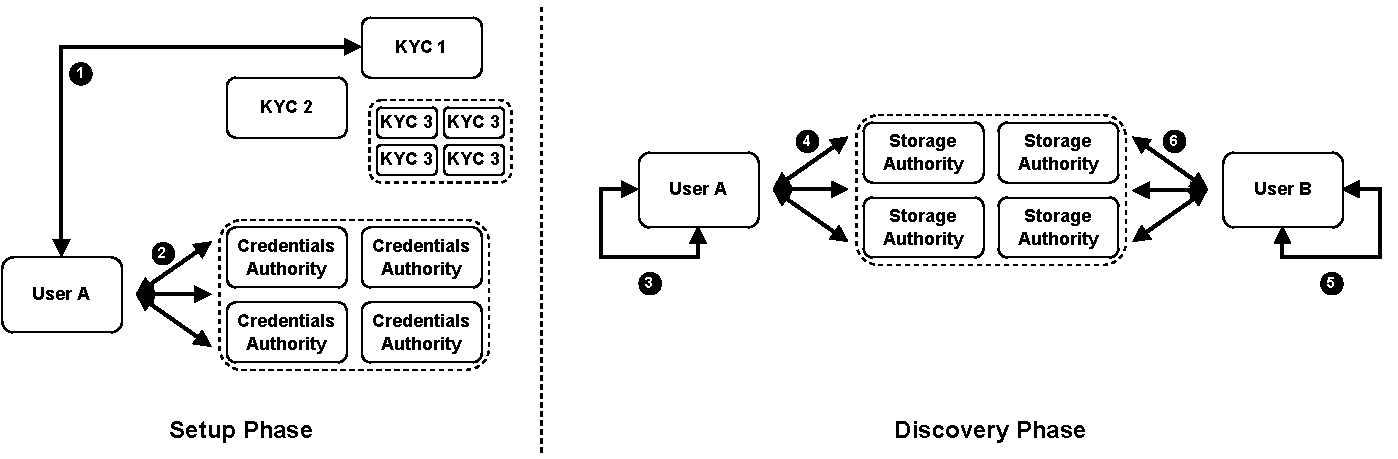
\includegraphics[width=\textwidth]{figures/arke-overview.drawio.pdf}
    \caption{
        $\sys$ overview. During the setup phase, users individually run a setup procedure with a registration authority to obtain an attestation over their identifier~(\one). They then use this attestation along with their blinded identifier to obtain a pair of long-term private keys by interacting with the key-issuing authorities~(\two). During the discovery phase, users locally derive a shared key with another user known by their identifier~(\three,\five) and use it to read and write the \sysname distributed store and discover their messages~(\four,\six).
    }
    \label{fig:arke-overview}
    \Description{}
\end{figure*}

\subsection{Design Goals} \label{sec:properties}
\sysname guarantees several system security, privacy, and performance properties.

\paragraph{System security properties}
\sysname maintains several systems security properties depending on which assumptions (\Cref{sec:assumptions}) hold. These security properties are formally defined and proved in \Cref{sec:security}.
\begin{itemize}
    \item \textbf{Validity:} A user $A$ can only update the \sysname store by updating the message associated with its identifier $n_A$.
    \item \textbf{Write consistency:} No correct storage authorities hold conflicting records.
    \item \textbf{Read consistency:} Two correct users cannot be tricked into reading different values. That is if user $B$ reads $\msg_A$ of user $A$ then user $C$ also reads $\msg_A$.
    \item \textbf{Write termination:} A correct user can eventually update the store to make its message discoverable.
    \item \textbf{Read termination:} A correct user can eventually read the store and learn the message associated with a user with a known identifier.
\end{itemize}

\paragraph{Privacy properties}
\alberto{Describe the privacy properties.}
\nico{A note on forward secrecy: as Arke is based on ID-NIKE, it does not provide forward secrecy (see Patterson and Srinivasan \cite{cryptoeprint:2007/453}). It is important that cryptographic applications such as Signal or blockchains only include "public" information in their Arke payloads to protect against future compromise of Arke private keys.}

\paragraph{Performance properties}
\sysname also guarantees the following system and performance properties. \Cref{sec:implementation_and_eval} demonstrates these properties through a thorough implementation and evaluation of \sysname.
\begin{itemize}
    \item \textbf{High-throughput:} \alberto{Show how many users we can support vs. how many users other solutions can handle (e.g. PSI-based scheme).}
    \item \textbf{Low-latency:} \alberto{Claim sub-second latency (even under load)?}
    \item \textbf{Performance under (crash-)faults:} The performance (throughput and latency) of \sysname is virtually unaffected by (crash-)faulty authorities. Note that evaluating a BFT system while experiencing Byzantine faults is an open research problem~\cite{twins}.
    \item \textbf{Linear scalability:} Authorities can take advantage of more hardware resources to linearly increase the system's throughput without impacting latency.
    \item \textbf{Bounded storage}: Storage is not growing linearly over time.
      \sysname enables authorities to periodically purge their store entries.
      This property is proven as part of \emph{consistency}.
\end{itemize}

\paragraph{Additional properties}
Furthermore, \sysname guarantees the following meta-properties:
\begin{itemize}
    \item \textbf{Censorship resistance}: Correct users can always obtain private keys from the key-issuing authorities. Furthermore correct users can write and read the \sysname store despite the presence of Byzantine authorities. This property is proved as part of \emph{write termination} and \emph{read termination}.
    \item \textbf{Authorities Non-Interactivity}: Neither the \sysname key-issuing authorities nor the storage authorities need to communicate with each other. This property allows for easier deployment and is crucial to integrate \sysname into the Sui blockchain~\cite{sui} (see \Cref{sec:instantiations}).
\end{itemize}

\subsection{Threat Model} \label{sec:assumptions}
We define the main assumptions under which \sysname guarantees the properties of \Cref{sec:properties}.

\assumption{Correct registration authorities}{\label{as:kyc}
    \sysname guarantees the security properties of \Cref{sec:properties} for identifiers issued by correct registration authorities. As mentioned in \Cref{sec:overview}, \sysname runs with a variety of registration authority. If a registration authority is malicious, it can only compromise the identifiers it attests to. That is, a corrupted registration authority \texttt{reg\_1} can compromise all interactions with identifiers of the form \texttt{user\_A@ref\_1} but the identifiers issued by other registration authority remain secure. A corrupt registration authority may attest to arbitrary bindings between users and identifiers.
}

\assumption{BFT authorities}{\label{as:bft}
    \sysname assumes a computationally bound adversary that controls the network and can corrupt at most $t$ key-issuing authorities and up to $f$ (out of $3f+1$) storage authorities in every epoch\footnote{\sysname requires quorum intersection only for the storage authorities.}. We say that authorities corrupted by the adversary are Byzantine or faulty and the rest are honest or correct. Byzantine authorities may act arbitrarily, while correct ones follow the protocol.
}

\assumption{Cryptography}{\label{as:crypto}
    The cryptographic schemes used in \sysname assume the existence of a non-degenerate and efficiently computable bilinear map $e: \GG_1 \times \GG_2 \rightarrow \GG_T$ for which the decisional bilinear Diffie-Hellman (DBDH) assumption holds. Hash functions are modeled as random oracles.
}

\assumption{Network model}{\label{as:net}
    To capture real-world networks we assume that links between users and correct authorities are reliable (the authorities do not communicate with each other). That is, all messages among the correct authorities eventually arrive. We assume a known $\Delta$ and say that execution of a protocol is eventually synchronous if there is a global stabilization time (GST) after which all messages sent among honest parties are delivered within the network delay $\Delta$ time. An execution is synchronous if GST occurs at time 0, and asynchronous if GST never occurs.
    %
    \sysname assumes an eventually synchronous network.
}

\assumption{Roughly synchronized clocks}{\label{as:clock}
    \sysname assumes that users have roughly synchronized clocks with the correct storage authorities.
    %That is, for every epoch $\Epoch$ of duration $\delta_e$, there is a period $0 < \delta \leq \delta_e$ during which the users and the correct authorities are in the same epoch $\Epoch$. Furthermore, all epochs have equal duration $\delta_e$. More formally:
    \begin{definition}[Roughly Synchronized Clocks]
      While a user is in epoch $e$, correct authorities are either in epoch $e$, $e-1$, or $e+1$. \philipp{We should probably use another notation for epochs to avoid confusion with bilinear maps.}
        Also, users remain in the same epoch each correct authority for a duration of at least $3\Delta$ (where $\Delta$ is the bound on message propagation time during periods of synchrony introduced in assumption 4).
        %Also, users and correct authority are both in epoch $e'$ for a duration of $\delta > 0$.
    \end{definition}
    % \alberto{Can we relax the assumption on "equal duration" and say that all users and correct authorities have epochs that last $\delta_e \pm \delta_e/2$?}
}

\section{Preliminaries} \label{sec:background}
	\paragraph{Notation} Let $\GG_1$, $\GG_2$ and $\GG_T$ be groups of prime order $q$ such that there exists an efficiently computable and non-degenerate bilinear map $e: \GG_1 \times \GG_2 \rightarrow \GG_T$.
	We denote by $g_1$, $g_2$, and $g_T$ the canonical generators of $\GG_1$, $\GG_2$, and $\GG_T$, respectively, and by $H: \{0,1\}^{\ast} \rightarrow \{0,1\}^l$, $H_1: \{0,1\}^{\ast} \rightarrow \GG_1$, and $H_2: \{0,1\}^{\ast} \rightarrow \GG_2$ hash functions.
	We treat $H$, $H_1$, and $H_2$ as random oracles. Let $\lambda$ denote a security parameter.

\subsection{Zero Knowledge Proofs}
	We make use of two types of zero knowledge proofs of knowledge (ZKPoK). 
	In both cases we consider non-interactive protocols.
	The generic interface for such protocols is defined below:
	
	\begin{definition}[Non-interactive ZKPoK]
		For a relation $\relation(\instance, \witness)$, a non-interactive ZKPoK is defined by three efficiently computable algorithms:
		\begin{itemize}
			\item $\zk.\setup(\pp) \rightarrow \pp_\zk$. Given some global public parameters $\pp$, output the $\zk$ public parameters $\pp_\zk$.
			\item $\zk.\prove(\pp_\zk, \instance, \witness) \rightarrow \pi$. Given the public parameters $\pp_\zk$ and instance-witness pair $(\instance, \witness) \in \relation$, output a proof $\pi$.
			\item $\zk.\verify(\pp_\zk, \instance, \pi) \rightarrow \{0, 1\}$. Given the public parameters, instance and proof, return $1$ if the proof is valid and $0$ otherwise.
		\end{itemize} 
		%
		The ZKPoKs that we use in \sysname have perfect completeness, zero-knowledge and simulation extractability. The latter is a strengthened notion of knowledge soundness, wherein the extractor must be successful even if the adversary is given access to simulated proofs.	
	\end{definition}

	\paragraph{Schnorr DLOG} For a group $\GG$ of prime order $q$, the Schnorr DLOG ZKPoK is a $\Sigma$-protocol for the relation 
	$$\relation_\dlog:= \left\{ ((x, y), \alpha): y = x^\alpha \right\}$$ 
	where $x, y \in \GG$ and $\alpha \in \ZZ_q$.

	\paragraph{ZKPoK for Hash Pre-images} We use a ZKPoK to keep users' identities private while still attesting that hashed values are correct. Let $\id$ be an identifier and $\alpha \in \ZZ_q$ a blinding factor, we define the relation $\relation_\ID$ as:
	$$\relation_\ID := \left\{ \left(\ID, (\id, \alpha)\right): \ID = \left(H_1(\id)^\alpha, H_2(\id)^\alpha \right) \right\}  $$
	For our benchmarks, we instantiate the ZKPoK for $\relation_\ID$ using the Groth16 zkSNARK \cite{groth2016size}.

\subsection{Distributed Key Generation}
 
	\paragraph{Key-expressible DKGs} A key-expressible DKG \cite{gurkan2021aggregatable} is a distributed key generation protocol which upholds a relaxed \emph{secrecy} property.
	Rather than require the existence of a simulator that outputs a target public key $\pk_1$, key-expressible DKGs only require that the simulator outputs a public key $\pk$ that can be expressed as a linear relation between the target key $\pk_1$ and a simulator-chosen key-pair $(\sk_2, \pk_2)$.
	As with classic DKGs, a key-expressible DKG involving $n$ participants is robust with respect to some threshold $t < n/2$ of malicious participants.
	
	Key-expressible DKGs can be used as a stand-in replacement for the key generation operation of certain protocols.
	In doing so, we obtain a threshold variant of the underlying protocol.
	Key-expressible DKGs preserve the security properties of the underlying protocol if that protocol is \emph{rekeyable} \cite{gurkan2021aggregatable}.

	\paragraph{Rekeyability} Informally, a protocol is said to be rekeyable if it is possible to transform objects (ciphertexts, signatures, etc...) that were formed using one set of keys into equivalent objects formed under a related set of keys.
	For example, a BLS signature under key $\sk_1$, $\sigma = H_1(m)^{\sk_1}$, can be transformed into a signature under the key $\alpha\sk_1 + \sk_2$ by computing $\sigma^\alpha \cdot H_1(m)^{\sk_2}$.
	A full formal definition is given in \cite{gurkan2021aggregatable}.


\subsection{Identity-Based Non-Interactive Key Exchange} \label{sec:idnike}

	\paragraph{Boneh-Waters ID-NIKE} We give a self-contained definition of the Boneh-Water ID-NIKE \cite{boneh2013constrained} adapted for our asymmetric pairing setting.
	
	\begin{definition}[Boneh-Waters ID-NIKE~\cite{boneh2013constrained}]
		The Boneh-Waters identity-based key exchange consists of three efficiently computable algorithms $\setup$, $\keygen$ and $\extract$ as follows:
		\begin{itemize}
			\item $\setup(\lambda)$: Choose a random $\msk \pick \ZZ_q$ and output $\msk$.
			\item $\extract(\msk, \id)$: compute $d_L = H_1(\id)^{\msk}$ and $d_R = H_2(\id)^{\msk}$. Output $sk_\id = (d_L, d_R)$
			\item $\sharedkey(sk_\id, \id')$: We assume that identifiers are lexicographically ordered. Output $k_{\id, \id'} = e(d_L, H_2(\id'))$ if $\id < id'$. Output $k_{\id, \id'} = e(H_1(\id'), d_R)$ if $\id > \id'$.
		\end{itemize}
		Note that $\sharedkey(\pp, sk_\id, \id') = \sharedkey(\pp, sk_\id', \id)$ for all $\id \neq \id'$ and $\pp$ generated by $\setup$.
	\end{definition}

	The security notion for such schemes is that of ``indistinguishability of shared keys" (IND-SK) and is formalised by Patterson and Srivinasan \cite{cryptoeprint:2007/453}.
	In the IND-SK game, an adversary can learn private keys for any identity or learn the shared symmetric key between any identity pairs by querying the $\extract$ and $\mathsf{Reveal}$ oracles respectively.
	At any moment, it may make a single query to a $\mathsf{Test}$ oracle for identities $\id_*$ and $\id'_*$.
	The oracle flips a bit $b$ and outputs $k_{\id_*, \id'_*}$ if $b = 0$ or a random element from $\GG_T$ if $b=1$.
	The adversary may still query the other two oracles (except on values $\id_*$ and $\id'_*$) and must eventually decide whether $b=0$ or $b=1$.
	Importantly the adversary may not query $\mathsf{Test}$ on any identity pairs for which it queried $\mathsf{Reveal}$ nor any identity for which it queried $\extract$.

	Boneh and Waters show that the ID-NIKE above is secure under the decision bilinear Diffie Hellman assumption in the random oracle model \cite{boneh2013constrained}.
	
\subsection{Authenticated Encryption with Associated Data (AEAD)}

	Authenticated Encryption with Associated Data (AEAD) is a symmetric key primitive that encrypts and authenticates a message.
	Furthermore, senders may choose to associate context data to the ciphertext in a way that is cryptographically binding.
	An AEAD scheme is defined by the following algorithms:
	
	\begin{itemize}
		\item $\aead.\enc_k(m, d) \rightarrow (c, \aeadtag)$. 
			Given a key $k$, message $m$ and associated data $d$, encrypt $m$ to produce the ciphertext $c$.
			Authenticate the associated data and ciphertext to produce a tag $\aeadtag$. 
			Output $(c, \aeadtag)$.
		\item $\aead.\dec_k(c, \aeadtag) \rightarrow m'$. 
			Given a key $k$, ciphertext $c$ and associated data $\aeadtag$, verify the authenticity of the associated data and ciphertext. 
			If the verification rejects, output $m' \leftarrow \perp$. 
			Otherwise decrypt $c$ and output $m' \leftarrow m$.
	\end{itemize}




\section{Contact Discovery Protocol}
\label{sec:contact_discovery_protocol}

The \sysname contact discovery protocol combines an ID-NIKE with an unlinkable handshake. 
The ID-NIKE allows users to establish shared secrets amongst each other knowing only their identifiers. 
Using this shared secret, they can run the unlinkable handshake to exchange arbitrary messages through an untrusted key-value store. 

In this section we describe a private and trust-minimised variant of the Boneh-Waters ID-NIKE, an unlinkable handshake protocol and show how to combine both to build a contact discovery protocol.

	\subsection{Threshold Oblivious ID-NIKE}
	
	The ID-NIKE as defined by Boneh and Waters \cite{boneh2013constrained} relies on a trusted third party to issue private keys to users.
	We modify their protocol to meet our privacy desiderata by (i) separating the key issuance operation into a registration and an extraction phase and, (ii) distributing the master secret key.  
	We call the resulting protocol a threshold and oblivious ID-NIKE.
	
	\paragraph{Oblivious Key Issuance} In the Boneh-Waters ID-NIKE, users must reveal their identifier to the trusted third party to obtain their secret key. 
	We separate this trusted party into two entities: a registration authority and a key-issuing authority. 
	We allow the registration authority to learn identifiers but not to compute their private keys. 
	Its role is to attest that a user $A$ owns a given identifier $\id_A$.
	On the other hand, the key-issuing entity is able to produce private keys but does not learn which identities they belong to.
	
	We replace the $\extract$ algorithm by four efficiently computable algorithms:
	\begin{itemize}
		\item $\register$
		\item $\blind$
		\item $\bextract$
		\item $\unblind$
	\end{itemize}
	\nico{TODO: describe each of these algorithms}
	
	\paragraph{Distributed Key Issuance} In the oblivious setting described above, the key-issuing authority is still all-powerful in that it is able to extract the private key of any identifier. To minimise the trust placed in the key-issuing authority, we distribute it into $n$ entities that each hold a share of the master secret key. Using a $(t, n)$-threshold DKG, we ensure that no single party can break the IND-SK property of the ID-NIKE as long as at most $t$ parties are corrupt.
	
	Distributing the key-issuing entity is enforced by replacing the $\setup_E$ algorithm by a DKG. The extraction algorithm is the same as $\bextract$ but is renamed to $\bpextract$ to emphasize the fact that it outputs blinded \emph{partial} secret keys. Finally we introduce the $\combine$ algorithm to reconstruct a secret key from a set of $t+1$ key shares.
	
%	We introduce an oblivious variant of the above ID-NIKE. 
%	An oblivious ID-NIKE allows to separate user key issuance into two parts: firstly a registration phase where users claim identities and then a blind key extraction phase.
%	Each phase depends on its own master secret key, denoted $\msk_R$ (registration) and $\msk_{E}$ (extraction) respectively.
%	The party performing registration learns the registered identity but is unable to extract its keys; on the other hand, the party performing the blind extraction can compute keys but learns nothing about the identity (other than the fact that it was previously registered).
%	
%	We then show that our oblivious ID-NIKE is rekeyable with respect to the key extraction master secret $\msk_E$ and is IND-SK secure.
%	We therefore instantiate an IND-SK secure \emph{threshold and oblivious} ID-NIKE using a key-expressible DKG.
%	The full protocol is described below:

	
	\begin{definition}[Threshold and Oblivious ID-NIKE]
		\label{def:tn_obl_idnike}
		Let $\Pi_\ID$ be a ZKPoK for the relation $\relation_\ID$.
		We define the $(t, n)$-threshold variant of the Boneh-Waters ID-NIKE as eight efficiently computable algorithms $\setup_E$, $\setup_R$, $\register$, $\blind$, $\bpextract$, $\unblind$, $\combine$ and $\sharedkey$ as follows:
		\begin{itemize}
			% Setup Extraction
			\item $\setup_E(\lambda, t, n)$: Participants $P_1, \dots , P_n$ execute a key-expressible DKG to compute Shamir secret shares $\msk_{E,1}, \dots , \msk_{E,n}$ of an (unknown) master secret key $\msk_E$.
				They jointly output a $\mathsf{transcript}$ and master public key $\mpk_E = (g_1^{\msk_E}, g_2^{\msk_E})$. Output $\msk_{E,i}$ to $P_i$ and $\pp \leftarrow (\mathsf{transcript}, \mpk_E)$.
			
			% Setup Registration
			\item $\setup_R(\lambda, \pp)$: choose a random registration secret key $\msk_R \pick \ZZ_q$ and compute the registration public key $\mpk_R = (g_1^{\msk_R}, g_2^{\msk_R})$. Output $\msk_R$ and $\pp \leftarrow \pp || \mpk_R$.
			
			% Register
			\item $\register(\msk_R, \id)$: compute $t_L = H_1(\id)^{\msk_R}$ and $t_R = H_2(\id)^{\msk_R}$. Output the registration token $t_\id \leftarrow (t_L, t_R)$.
	
			% Blind
			\item $\blind(\pp, \id, t_\id)$:
			choose a random blinding factor $\alpha \pick \ZZ_q$.
			Compute 	
			\begin{equation}
				\begin{aligned}
					\ID &\leftarrow \left(H_1(\id)^\alpha, H_2(\id)^\alpha \right) \\
					\pi_\ID &\leftarrow \Pi_\ID.\prove(\pp_\zk, \ID, (\id, \alpha)) \\
					\widehat{t_\id} &\leftarrow {t_\id}^\alpha 
				\end{aligned} 
			\end{equation}
			Output a blinded identifier $\widehat{\id} \leftarrow (\ID, \pi_\ID)$, blinded registration token $\widehat{t_\id}$ and the blinding factor $\alpha$.
			
			% Blind Partial Extract
			\item $\bpextract(\msk_{E,i}, \pp, \widehat\id, \widehat{t_\id})$: 
				Parse $\widehat\id$ as $(\ID, \pi_\ID)$, and $\widehat{t_\id}$ as $(\widehat{t_L}, \widehat{t_R})$.
				Parse $\ID$ as $(\ID_L, \ID_R)$.
				Check that the following equations hold:
				\begin{equation}
						\begin{aligned}
							\pairing{\widehat{t_L}}{g_2} &\stackrel{?}{=} \pairing{\ID_L}{{g_2}^\msk} \\
							\pairing{g_1}{\widehat{t_R}} &\stackrel{?}{=} \pairing{{g_1}^\msk}{\ID_R} \\
							\Pi_\ID.\verify(\pp_\zk, \ID, \pi_\ID) &\stackrel{?}{=} 1 \quad \text{(accept)}
						\end{aligned}
				\end{equation}
				%
				If all equations verify successfully, compute and return a blinded partial key $\widehat {sk_{\id, i}} \leftarrow \ID^{\msk_E}$, else return $\perp$.
			
			% Unblind
			\item $\unblind(\widehat {sk_{\id, i}}, \alpha)$: compute and output the partial key ${sk_{\id, i}} \leftarrow \widehat {sk_{\id, i}}^{\frac{1}{\alpha}}$.
			
			% Combine
			\item $\combine(\left\{sk_{\id, i} \right\}_{i =1}^{t+1})$: using a set of $t+1$ valid partial keys, compute $d_L$ and $d_R$ using Lagrange interpolation ``in the exponent''.
			 	Let $L_i$ denote the Lagrange coefficient for the $i$-th share in the given set, $d_L = \prod_{i = 1}^{t+1} {d_{L, i}}^{L_i}$ and $d_R = \prod_{i = 1}^{t+1} {d_{R, i}}^{L_i}$. 
			 	\footnote{As required, $d_L = \prod_{i = 1}^{t+1} {d_{L, i}}^{L_i} = H_1(\id)^{\sum_{i = 1}^{t+1}\msk_{E,i}L_i} = H_1(\id)^{\msk_E}$}.
			 	Output the user key $sk_\id = (d_L, d_R)$.
			
			% Shared Key
			\item $\sharedkey(sk_\id, \id')$: We assume that identifiers are lexicographically ordered. Output $k_{\id, \id'} = e(d_L, H_2(\id'))$ if $\id < \id'$. Output the shared key $k_{\id, \id'} = e(H_1(\id'), d_R)$ if $\id > \id'$.
		\end{itemize}
		It holds that $\sharedkey(\pp, sk_\id, \id') = \sharedkey(\pp, sk_\id', \id)$ for all $\id \neq \id'$ and $\pp$ generated by $\setup_E$.
	\end{definition}
	
	\paragraph{IND-SK Security} We show that the threshold and oblivious ID-NIKE described here is IND-SK secure under the DBDH assumption in the random oracle model if $\Pi_\ID$ is simulation extractable.
	
	\begin{theorem}
	\label{theorem:threshold_oblivious_idnike_security}
		The threshold and oblivious ID-NIKE of \Cref{def:tn_obl_idnike} is IND-SK under the DBDH assumption when modelling the functions $H_1$, $H_2$ as random oracles and if $\Pi_\ID$ is simulation extractable.
	\end{theorem}
	
	\noindent \textit{Proof intuition.} We first show that the security of the oblivious variant of the ID-NIKE reduces to that of the Boneh-Waters ID-NIKE assuming that $\Pi_\ID$ is simulation extractable. Indeed if an adversary $\adv$ can break the IND-SK security of the oblivious ID-NIKE, then we can build an adversary $\bdv$ that breaks the Boneh-Waters ID-NIKE. Informally, $\bdv$ takes on the role of the registration authority and can emulate the key-issuing authority. It does so by using the extractor for $\Pi_\ID$ to effectively ``remove the blinding'' on $\adv$'s requests to its $\bextract$ oracle. Since $\Pi_\ID$ is simulation extractable, the extractor will succeed with overwhelming probability.
		
	The second step it to show that the oblivious ID-NIKE is rekeyable with respect to the master secret key $\msk_E$. We do so using similar techniques as those used in \cite{gurkan2021aggregatable} for BLS signatures. 
	
	Finally we show that key-expressible DKGs are security preserving for rekeyable ID-NIKEs, allowing us to transform the oblivious ID-NIKE into a threshold and oblivious ID-NIKE under the same security assumptions. Combining the above with the already proven security of the Boneh-Waters ID-NIKE proves our theorem. $\square$
	
	\subsection{Unlinkable Handshake}
	
	\paragraph{Unlinkability}
	
	\paragraph{Bounded Storage}
	
	\subsection{The \sysname Protocol}
	
	\paragraph{Setup Phase}
	
	\paragraph{Discovery Phase}
	
	
	
	
	
	
	
	
	
	
	
\section{The \sysname Key-Value Store}
\label{sec:store}

In this section we realise a distributed and consistent key-value store that fulfils the required properties for the \sysname protocol without the need for a consensus protocol.

\nico{TODO, go through this section and fix language and references to make sense in the new structure}

\subsection{Read and Write Protocol} \label{sec:read-write}
\Cref{fig:arke-store} presents an overview of the protocol allowing user $A$ to respectively write and read the key-value pairs $(\key_{AB}, \val_{AB})$ and $(\key_{BA}, \val_{BA})$ from the store.

\begin{figure*}[t]
    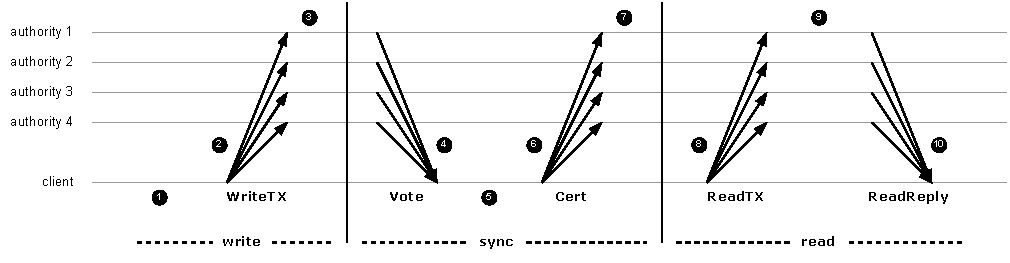
\includegraphics[width=\textwidth]{figures/arke-store.drawio.pdf}
    \caption{Example of \sysname write (\one-\three), sync (\four-\seven), and read (\eight-\ten) protocol with 4 authorities.}
    \Description{}
    \label{fig:arke-store}
\end{figure*}

\paragraph{Writing the store}
Steps \one-\three of \Cref{fig:arke-store} illustrate the high-level interactions between user $A$ and the storage authorities to allow the user to write the distributed store.
%
User $A$ uses its writing tag $t_{AB}$ (\Cref{sec:key-derivation}) as a private signing key to create and sign a \emph{write transaction}. This transaction mutates (or creates) the key-value pair $(\key_{BA}, \val_{BA}) = (g_1^{t_{BA}}, c_{BA})$ of the \sysname store~(\one).
%
The user transaction is then sent to each \sysname storage authority~(\two).
%
The authorities check it for validity and lock the store entry to mutate~(\three). The write operation is completed as soon as $2f+1$ authorities successfully terminate this step. \Cref{alg:process-tx} of \Cref{sec:store-operations} describes in details how authorities process incoming write transactions.

\paragraph{Synchronization}
Steps \four-\seven of \Cref{fig:arke-store} illustrate the store synchronization step. At this stage, user signature keys are not needed anymore, and the synchronization process may be performed by any user client or third-party synchronizer process. Storage authorities always provide idempotent replies to protocol messages: it is safe to send multiple times the same message to an authority.
%
After processing a write transaction, each authority returns a \emph{vote} to the user or synchronizer process~(\four).
%
The user collects the votes from a quorum of $2f+1$ authorities to form a \emph{certificate}~(\five).
%
The certificate is then sent back to all validators~(\six).
%
The authorities check the certificate and upon success mutate the specified store entry and release the locks to allow future updates~(\seven). \Cref{alg:process-cert} of \Cref{sec:store-operations} describes this step in details.
%
The write and synchronization mechanisms can be seen as the ‘Signed Echo Broadcast’ implementation of a Byzantine consistent broadcast on the label $(\key_{BA}, \Version)$~\cite{cachin2011introduction}.

\paragraph{Reading the store}
Steps \eight-\ten of \Cref{fig:arke-store} illustrate the minimal interactions between user $A$ and the storage authorities to allow the user to read the distributed store.
%
The user creates a \emph{read transaction} to read the value $\val_{BA} = c_{BA}$ associated with a specified store entry $\key_{BA} = g_1^{t_{BA}}$~(\eight).
%
Each authority replies with a \emph{read reply} containing the latest value they hold for that store entry or $\None$ if the entry is not in their store~(\nine).
%
Finally, user $A$ processes the replies, performs the synchronization protocol described above (in case it did not terminate), and deduces the latest value associated with the queried key~(\ten). \Cref{alg:process-reply} of \Cref{sec:store-operations} describes in details how readers process incoming read replies.

\paragraph{Rate limiting} We introduce anonymous rate limiting in order to prevent a malicious user from overloading the store with SPAM writes. Users are allowed a fixed number of store writes per epoch; any further attempts to write should be prevented and optionally incur a punishment. Such a mechanism can be implemented using PrivacyPass: users (or their client-side software) periodically authenticate to their registration authority and request PrivacyPass tokens which they can later redeem at each store write. PrivacyPass has the advantage of using lightweight cryptography and is in the process of being standardized by the IETF. On the other hand, it does not allow to identify cheaters as would be the case with other, more cryptographic-intensive approaches.

Importantly, breaching the rate limit or setting the policy to allow too many writes does not threaten user privacy. Indeed discovery in \sys is a bidirectional process and the handshake is only completed if \textit{both} parties participate.
\nico{TODO cite privacy pass, RLN and the "How to Win the Clone Wars" paper}
~\cite{camenisch2006how,davidson2018privacy}

\subsection{Protocol Messages and Data Structures} \label{sec:protocol-messages}
\sysname storage authorities and users run the read and write protocol described in \Cref{sec:read-write} by exchanging the following messages:
\begin{itemize}
    \item A \emph{write transaction} ($\tx$) is a structure sent by user $A$ to the storage authorities to update a specific store entry. The transaction is signed by user $A$ using the tag $t_{AB}$ as the secret key and contains the following fields:
          \begin{itemize}
              \item The value $\val_{AB} = c_{AB}$ to write on the store.
              \item The location of the store $\key_{AB} = g_1^{t_{AB}}$ where to write.
              \item A version number ensures the freshness of the transaction.
              \item The current epoch number.
              \item A signature by $t_{AB}$ over the transaction's fields.
          \end{itemize}
          The transaction also supports a few self-explanatory access operations, such as $\version{\tx}$ to get its version number and functions to access the key-value pair to update.

    \item A \emph{vote} (\vote) on a write transaction contains the transaction itself as well as the identifier and signature of a store authority.

    \item A \emph{certificate} ($\cert$) on a write transaction contains the transaction itself as well as the identifiers and signatures from at least a quorum of $2f+1$ storage authorities. A certificate may not be unique, and the same logical certificate may be signed by a different quorum of storage authorities. However, two different valid certificates on the same transaction are treated as representing semantically the same certificate. The identifiers of signers are included in the certificate (i.e., accountable signatures~\cite{boneh2018compact}) to identify validators ready to process the certificate. Similarly to transactions, certificates support several self-explanatory access functions to get its version number and the key-value pair to update.

    \item A \emph{read transaction} ($\readtx$) is a structure specifying a store entry $\key_{BA} = g_1^{t_{BA}}$ to read.

    \item A \emph{read reply} ($\reply$) on a read transaction contains the transaction itself as well as the latest tuple $(\cert, \vote)$ known by a store authority. It also contains the identifier and signature of that authority.
\end{itemize}

Each store authority maintains two persistent tables abstracted as key-value maps, with the usual $\mathsf{contains}$, $\mathsf{get}$, and $\mathsf{set}$ operations.

\begin{itemize}
    \item The \emph{lock map} records the last valid update to a store entry embedded in the last valid certificate $\cert$ seen by the authority. It also stores the last vote $\vote$ that the authority generated to further update the key. Alternatively, it may hold $\None$ if the store entry does not exist or the authority did not see the transaction before. The lock map is defined as follows:
          $$\lockdb[\storekey{\tx}] \rightarrow (\cert, \Vote \textsf{Option})$$
\end{itemize}


\subsection{Store Core Operations} \label{sec:store-operations}
We detail the operations performed by the authorities when receiving write transactions and certificates from users and describe how users process read replies from the authorities.

\paragraph{Process write transaction}
\Cref{alg:process-tx} shows how storage authorities process write transactions; that is, step~\three of \Cref{fig:arke-store} (see \Cref{sec:read-write}).
%
Upon receiving a write transaction $\tx$ the storage authority calls \textsc{ProcessTx} to perform several checks:
\begin{itemize}
    \item \textbf{Check (\ref{alg:process-tx}.1):} It ensures that the author of  $\tx$ is authorized to write in the specified store location. That is, check that $\tx$ is correctly signed using the secret key corresponding to the public key $\Key_{AB} = g_1^{t_{AB}}$ included in the transaction as the public key.
    \item \textbf{Check (\ref{alg:process-tx}.2):} It tries to acquire a (mutex) guard over the store entry $\storekey{\tx}$; otherwise, it returns an error and terminates the processing of $\tx$. Acquiring a guard ensures that no other task can concurrently perform the next step of the algorithm on the same key.
    \item \textbf{Check (\ref{alg:process-tx}.3):} It ensures the transaction is for the current epoch $\Epoch$. This check is crucial to maintain consistency across epochs as the $\lockdb$ store is partially reset upon epoch change (see \Cref{sec:epoch-change}).
    \item \textbf{Check (\ref{alg:process-tx}.4):} It ensures the version number of $\tx$ is the next natural integer expected in the sequence (\Cref{alg:line:expected_version}). If it is the first time the authority writes this store entry (i.e., $\lockdb[\key]$ is empty), the value $\OldCert$ at \Cref{alg:line:load_key} is a placeholder certificate without content and with version number zero; and $\Vote = \None$.
    \item \textbf{Check (\ref{alg:process-tx}.5):} It checks that $\lockdb[\storekey{\tx}]$ is either $\None$ or set to \emph{the same} transaction $\tx$, and atomically sets it to $\vote$. In other words, no other transaction $\tx' \neq \tx$ has been signed for the same version number. This is an important validity check to implement \emph{byzantine consistent broadcast}~\cite{cachin2011introduction} and ensure safety.
\end{itemize}
If all checks are successful then the authority returns a vote $\vote$, i.e., a signature on the write transaction. Processing a transaction is idempotent upon success, and always returns a vote (\vote) within the same epoch. Any party may collate a transaction and votes (\vote) from a quorum of $2f+1$ authorities of epoch $\Epoch$, to form a certificate $\cert$.
%
Many tasks can call \textsf{ProcessTx} concurrently (or in parallel). \sysname only acquires mutexes\footnote{
    This mutex ensures that correct authorities never return two different votes over the same store entry update. The following scenario may happen if we omit the mutex \Cref{alg:line:acquire_tx_guard}. Two different transactions ($\tx$ and $\tx'$) updating the same store entry (with the same version) may be submitted concurrently to the authority. Both transactions pass all checks until \Cref{alg:line:assign_lock}. The first transaction then assigns the lock \Cref{alg:line:assign_lock} and the authority returns $\vote$; the second transaction then overwrites the lock and the validator returns a conflicting $\vote'$.
}
on the minimum amount of data: the store entry that the transaction is trying to update (\Cref{alg:process-tx} \Cref{alg:line:acquire_tx_guard}).

\begin{algorithm}[t]
    \caption{Process $\tx$}
    \label{alg:process-tx}
    \small
    \begin{algorithmic}[1]
        \Statex // Executed upon receiving a write transaction from a user.
        \Statex // Many tasks can call this function concurrently.
        \Procedure{ProcessWriteTx}{$\tx$}
        %
        \State // Check (\ref{alg:process-tx}.1): Check the transaction's validity (see \Cref{sec:store-operations}).
        \If{!$\valid{\tx}$} \Return Error \EndIf
        \State
        %
        \State // Check (\ref{alg:process-tx}.2): Try to acquire a mutex over $\storekey{\tx}$
        \State $\Key \gets \storekey{\tx}$
        \State guard = \Call{AcquireGuard}{$\Key$} \Comment{Error if cannot acquire guard} \label{alg:line:acquire_tx_guard}
        \State
        %
        \State // Check (\ref{alg:process-tx}.3): Ensure $\tx$ is for the current epoch \Epoch.
        \If{$\epoch{\tx} \neq \Epoch$} \Return Error \EndIf
        \State
        %
        \State // Check (\ref{alg:process-tx}.4): Check $\tx$'s version.
        \State $(\OldCert, \Vote) \gets \lockdb[\Key]$ \Comment{$\None$ if $\Key$ is missing} \label{alg:line:load_key}
        \State $\Version \gets \version{\OldCert} + 1$ \Comment{Expected version} \label{alg:line:expected_version}
        \If{$\Version \neq \version{\tx}$} \Return Error \EndIf
        \State
        \State // Check (\ref{alg:process-tx}.5): Only sign non-conflicting transactions.
        \State $\vote \gets \signtx{\tx}$
        \If{$\Vote == \None$} \label{alg:line:check_none_vote}
        \State $\lockdb[\Key] \gets (\OldCert, \vote)$ \label{alg:line:assign_lock}
        \ElsIf{$\Vote \neq \vote$} \label{alg:line:check_different_vote}
        \State \Return Error \label{alg:line:no_conflict}
        \EndIf
        \State
        %
        % \State $\vote \gets \signtx{\tx, \Epoch}$
        % \If{$\lockdb[\Key] == \None$}
        % \State // Check (\ref{alg:process-tx}.3): Ensure $\tx$'s version is 1.
        % \If{$\version{\tx} \neq 1$} \Return Error \EndIf
        % \State $\lockdb[\Key] \gets (\Genesis, \vote)$
        % \Else
        % \State $(\OldCert, \Vote) \gets \lockdb[\Key]$ \label{alg:line:expected_version}
        % \State
        % \State // Check (\ref{alg:process-tx}.4): Check $\tx$'s version.
        % \State $\Version \gets \version{\OldCert} + 1$ \Comment{Expected version}
        % \If{$\Version \neq \version{\tx}$} \Return Error \EndIf
        % \State
        % \State // Check (\ref{alg:process-tx}.5): Only sign non-conflicting transactions.
        % \If{$\Vote == \None$}
        % \State $\lockdb[\Key] \gets (\OldCert, \vote)$ \label{alg:line:assign_lock}
        % \ElsIf{$\Vote \neq \vote$}
        % \State \Return Error
        % \EndIf
        % \EndIf
        % \State
        %
        \State // Return a vote on $\tx$.
        \State \Return \vote
        \EndProcedure
    \end{algorithmic}
\end{algorithm}

\paragraph{Process write certificates}
\Cref{alg:process-cert} shows how storage authorities process write certificates; that is, step~\seven of \Cref{fig:arke-store} (see \Cref{sec:read-write}).
%
Upon receiving a certificate $\cert$ a \sysname authority calls \textsf{ProcessCert} of \Cref{alg:process-cert} to perform a number of checks:
\begin{itemize}
    \item \textbf{Check (\ref{alg:process-cert}.1):} It ensures the certificate is signed by a quorum of $2f+1$ authorities. Optionally, the authority may re-check that the writer is authorized to update the specified store entry (check (\ref{alg:process-tx}.1)); if they aren't the certificate $\cert$ is proof of catastrophic failure and that the BFT assumption broke.
    \item \textbf{Check (\ref{alg:process-cert}.2):} It tries to acquire a guard over the store entry $\storekey{\cert}$; otherwise, it returns an error and terminates the processing of $\cert$. Acquiring a guard ensures that no other task can concurrently perform the next step of the algorithm on the same key, or call \textsc{ProcessWriteTx} (\Cref{alg:process-tx}) with a new transaction over the same store entry $\storekey{\cert}$.
    \item \textbf{Check (\ref{alg:process-cert}.3):} It ensures the certificate is for the current epoch $\Epoch$. This check is crucial to maintain consistency across epochs as the $\lockdb$ store is partially reset upon epoch change (see \Cref{sec:epoch-change}).
    \item \textbf{Check (\ref{alg:process-cert}.4):} It ensures that $\cert$ is newer than the latest certificate seen by the authority. This check ensures the state of the authority cannot be reverted by replaying older certificates.
\end{itemize}

If all check succeeds, the value associated with the store entry $\storekey{\cert}$ is updated to $\storevalue{\cert}$ and the version number expected for the next update to $\version{\cert}$. These two operations are implicitly performed at \Cref{alg:line:update-store}: the latest value and version of $\storekey{\cert}$ are persisted as part of the certificate $\cert$. Further, the lock previously set to $\Vote$ is now released in order to accept future updates of $\storekey{\cert}$.

\begin{algorithm}[t]
    \caption{Process $\cert$}
    \label{alg:process-cert}
    \small
    \begin{algorithmic}[1]
        \Statex // Executed upon receiving a write certificate from a user.
        \Statex // Many tasks can call this function concurrently.
        \Procedure{ProcessWriteCert}{$\cert$}
        %
        \State // Check (\ref{alg:process-cert}.1): Check the certificate's validity (see \Cref{sec:store-operations}).
        \If{!$\valid{\cert}$} \Return Error \EndIf
        \State
        %
        \State // Check (\ref{alg:process-cert}.2): Try to acquire a mutex over $\storekey{\tx}$
        \State $\Key \gets \storekey{\tx}$
        \State guard = \Call{AcquireGuard}{$\Key$} \Comment{Error if cannot acquire guard} \label{alg:line:acquire_tx_guard}
        \State
        %
        \State // Check (\ref{alg:process-cert}.3): Ensure $\cert$ is for the current epoch \Epoch.
        \If{$\epoch{\cert} \neq \Epoch$} \Return Error \EndIf \label{alg:line:cert-epoch-check}
        \State
        %
        \State // Check (\ref{alg:process-cert}.4): Check $\cert$'s version.
        \State $(\OldCert, \Vote) \gets \lockdb[\Key]$ \Comment{$\None$ if $\Key$ is missing} \label{alg:line:load_cert}
        \State $\Version \gets \version{\OldCert}$ \Comment{Expected version}
        \If{$\Version < \version{\cert}$} \label{alg:line:check-cert-version}
        \State $\lockdb[\Key] \gets (\cert, \None)$ \Comment{Write $\storevalue{\cert}$} \label{alg:line:update-store}
        \EndIf
        \State
        \State \Return $Ack$ \Comment{Acknowledgement certificate processing}
        \EndProcedure
    \end{algorithmic}
\end{algorithm}

\paragraph{Process read replies}
\Cref{alg:process-reply} shows how the reader processes read replies received from a quorum of storage authorities; that is, step~\ten of \Cref{fig:arke-store} (see \Cref{sec:read-write}). The reader collects at least $2f+1$ read replies $[\reply]$.
%
Check (\ref{alg:process-reply}.1) filters out
\begin{enumerate}
    \item Any malformed or empty reply. Malformed replies do not contain valid authorities' signatures and empty replies contain $(\cert, \vote) = (\None, \None)$.
    \item Any reply concerning protocol messages with epoch number $e$ such that $e + E \leq \Epoch$. The parameter $E$ is the maximum number of epochs for which the storage authorities keep a store entry, and $\Epoch$ is the current epoch of the reader.
\end{enumerate}
After this check, if the set $[\reply]$ is empty replies, the reader reads $\None$ (\Cref{alg:line:read_none}).
%
Alternatively, the reader looks for the highest certificate and the highest valid vote (\Cref{alg:line:search_highest}). These are simply the certificate and valid vote included in the set $[\reply]$ with the highest version. A valid vote contains a $\tx$ that passes Check (\ref{alg:process-tx}.1) of \Cref{alg:process-tx}.
%
Finally, the reader compares the highest certificate $\cert$ with the highest vote $\vote$. If the certificate has a higher version than the vote, the reader optionally disseminates the certificate to any authority who missed it (\Cref{alg:line:disseminate_cert}) and then reads $\storevalue{\cert}$.
%
Alternatively, the reader concludes that further authority synchronization is needed (\Cref{alg:line:finishg_sync}). It then performs the synchronization steps \four-\seven of \Cref{fig:arke-store} described in \Cref{sec:read-write}, or waits for another party to synchronize the authorities. The reader then re-tries the read operation.


\begin{algorithm}[t]
    \caption{Process $\reply$}
    \label{alg:process-reply}
    \small
    \begin{algorithmic}[1]
        % \Statex // Extract the highest $\cert$ and $\vote$.
        % \Function{HigestReply}{$[\reply]$}
        % \State $(\HighestCert, \HighestVote) \gets (\None, \None)$
        % \State $\HighestVoteCount \gets 0$
        % \State
        % \For{$\reply \in [\reply]$}
        % \State $(\cert, \vote) \gets \reply$
        % \If{$\cert > \HighestCert$}
        % \State $\HighestCert \gets \cert$
        % \EndIf
        % \If{$\vote = \HighestVote$}
        % \State $\HighestVoteCount \gets \HighestVoteCount + 1$
        % \ElsIf{$\vote > \HighestVote$}
        % \State $\HighestVote \gets \Vote$
        % \State $\HighestVoteCount \gets 1$
        % \EndIf
        % \EndFor
        % \State
        % \If{$\HighestVoteCount \geq f+1$}
        % \State \Return $(\HighestCert, \HighestVote)$
        % \Else
        % \State \Return $(\HighestCert, \None)$
        % \EndIf
        % \EndFunction

        \Statex
        \Statex // Executed upon receiving read replies from an authority.
        \Procedure{ProcessReadReply}{$[\reply]$}
        \State // Check (\ref{alg:process-reply}.1): Filter out invalid replies (see \Cref{sec:store-operations}).
        \State $[\reply] \gets \valid{[\reply]}$
        \State
        %
        \If{$![\reply]$} \Comment{If the reply set is empty}
        \State \Return $\None$ \label{alg:line:read_none}
        \EndIf
        \State
        %
        \State $(\cert, \vote) \gets \Call{HigestReply}{[\reply]}$ \label{alg:line:search_highest}
        \If{$\cert \geq \vote$}
        \State $\Call{DisseminateCert}{\cert}$ \Comment{Optional} \label{alg:line:disseminate_cert}
        \State \Return $\storevalue{\cert}$ \label{alg:line:read_cert}
        \Else
        \State $\tx \gets \transaction{\vote}$
        \State \Return $\Call{FinishSync}{\tx}$ \Comment{Finish sync operation} \label{alg:line:finishg_sync}
        \EndIf
        \EndProcedure
    \end{algorithmic}
\end{algorithm}


% \alberto{
%     Check 3.1 rejects replies with epoch $e + E \leq \Epoch$. Validators only delete with $\epoch{\cert} < e + E$. Read consistency depends on the offset of one epoch between check (3.1) and the deletion of $\cert$.

%     %
%     Reader $r_1$ in epoch $e$ reads from $v_1$ and gets $\cert$; then $v_1$ enters $e$ and deletes $\cert$; finally reader $r_1$ in epoch $e$ reads from $v_1$ and does not get $\cert$.
%     %
%     If $v_1$ deletes $\cert$ in epoch $e$ it means  $\epoch{\cert} < e + E$. However $r_1$ only accepts $\epoch{\cert} \geq e + E$, hence a contradiction.
% }

% \alberto{Remember, readers only read from certificates (not votes); so overlaps over votes do not matter.}


\subsection{Epoch Change} \label{sec:epoch-change}
Epoch changes serve two main purposes, they allow unlocking any store entry partially written by faulty writers and they are used to clean up storage by deleting hold entries.

\paragraph{Transactions unlocking}
A faulty writer may sign two conflicting transactions $\tx$ and $\tx'$ with the same version number and both updating the same store entry $\Key = \storekey{\tx} = \storekey{\tx'}$. It is then possible that a set of $f+1$ correct authorities process $\tx$ and lock $\lockdb[\Key] \gets (\OldCert, \vote)$ (\Cref{alg:line:assign_lock} of \Cref{alg:process-tx}), and the other $f$ correct authorities process $\tx'$ and lock $\lockdb[\Key] \gets (\OldCert, \vote')$. As a result, there may never be a certificate neither over $\tx$ nor over $\tx'$. The store entry $\Key$ is then effectively locked forever.

\sysname allows unlocking $\Key$ at the end of every epoch by dropping all locks. That is, authorities forget all votes they issued during the epoch. Authorities set $\lockdb[\Key] \gets (\OldCert, \None)$ for every entry in their store\footnote{
    This operation may be performed lazily at runtime to avoid the cost of iterating through the store upon every epoch change.
}.
%
Intuitively, dropping all locks at epoch change is safe because check (\ref{alg:process-cert}.3) of \Cref{alg:process-cert} ensures certificates are only valid for a single epoch (see \Cref{sec:security}).

\paragraph{Storage cleanup}
One of the main properties of \sysname is its ability to clean up storage after long periods of inactivity. Correct authorities delete keys that have not been updated in the last $E$ epochs. That is, they drop the store entries $\lockdb[\Key]$ for every entry $\Key$ associated with a certificate $\cert$ where $\epoch{\cert} + E < \Epoch$ (where $\Epoch$ is the current epoch).
%
This operation is performed asynchronously and lazily at runtime to avoid the cost of iterating through the store upon epoch change. Upon loading the latest certificate from storage (\Cref{alg:line:load_cert} \Cref{alg:process-cert}), the store $\lockdb$ returns $\None$ if $\OldCert$ should be deleted.
%
Intuitively, this operation is safe (see \Cref{sec:security}) because readers only consider a certificate $\cert$ if $\epoch{\cert} + E > \Epoch$ (check (\ref{alg:process-reply}.1) of \Cref{alg:process-reply}), and it preserves liveness because readers and correct authorities are in the same epoch $\Epoch$ for a duration $\delta > 0$ (i.e., correct authorities have roughly synchronized clocks, see \Cref{sec:assumptions}).



\subsection{Scaling the \sysname Store}
\sysname scales and achieves high performance with two main strategies: (i) authorities can process multiple transactions and certificates in parallel, and (ii) they can take advantage of more hardware to further increase throughput.

\paragraph{Scaling on multiple cores}
\Cref{alg:process-tx} and \Cref{alg:process-cert} are designed to take advantage of all the CPU cores available on the authority machine. This is achieved by taking a simple guard on the store entry to update (rather than on the entire state) and processing non-conflicting updates in parallel. Both functions \textsc{ProcessWriteTx} (\Cref{alg:process-tx}) and \textsc{ProcessCert} (\Cref{alg:process-cert}) can be called by multiple tasks.

\paragraph{Scaling on multiple machines}
storage authorities can scale and arbitrarily increase their throughput by using more hardware. That is, rather than limiting each authority to operate on a single server, they could operate on a rack or even an entire data center.
%
\sysname requires no state sharing between the machines of the authority, and thus allows for a very efficient sharding at each authority by key. Each machine is responsible to handle write, sync, and read operations only on a predefined subset of the keys. The consistent broadcast channel implementing the write operation is executed on a per-entry basis. Therefore, the protocol does not require any state sharing between shards. \Cref{sec:implementation_and_eval} illustrates how storage authorities take advantage of multiple machines to linearly increase their throughput.

\section{Security} \label{sec:security}
We argue that \sysname satisfies the security and privacy properties defined in \Cref{sec:properties} under the assumptions defined in \Cref{sec:assumptions}.

\subsection{Key Derivation Security} \label{sec:key-derivation-security}
The security of the \sysname key derivation protocol (\Cref{sec:key-derivation}) relies on assumption~\ref{as:crypto} (cryptography) defined in \Cref{sec:assumptions}.
%
The correctness of the key derivation process is essential to ensure the \emph{termination} properties of \sysname (\Cref{sec:termination}), and its privacy property are essential to guarantee \emph{validity} (\Cref{sec:validity}) and \emph{unlinkability} (\Cref{sec:unlinkability}).

\begin{theorem}[Key Derivation Correctness] \label{th:key-derivation-correctness}
    Two correct users $A$ and $B$ running the \sysname key derivation protocol (\Cref{sec:key-derivation}) with each other's username derive the same shared key $k$ and tags $t_{AB}$ and $t_{BA}$.
\end{theorem}
\begin{proof}
    \missing{Crypto proof}
\end{proof}

\begin{theorem}[Key Derivation Privacy] \label{th:key-derivation-privacy}
    At the end of the \sysname key derivation protocol (\Cref{sec:key-derivation}), only user $B$ and user $C$ learn their shared key $k_{BC}$ and the tags $t_{BC}$ and $t_{CB}$.
\end{theorem}
\begin{proof}
    \missing{Crypto proof}
\end{proof}


\subsection{Validity} \label{sec:validity}
The validity of \sysname relies on assumption~\ref{as:bft} (BFT) and assumption~\ref{as:crypto} (cryptography)  defined in \Cref{sec:assumptions}. \sysname can avoid relying on the BFT assumption for validity if we augment \Cref{alg:process-cert} (\Cref{sec:store-operations}) to (re-)run Check (\ref{alg:process-tx}.1) of \Cref{alg:process-tx} upon processing certificates (see \Cref{sec:store-operations}).

\paragraph{Authenticated writes}
We start by showing that users can only update the \sysname store at locations associated with their own username. That is, malicious users cannot interfere with the discovery protocol of other users.

\begin{lemma} \label{th:autenticated-tx-processing}
    No correct storage authority issues a vote $\vote$ over a transaction $\tx$ writing the \sysname store at a location $\key_{BC}=g_1^{t_{BC}}$ if the transaction's author does not know $t_{BC}$.
\end{lemma}
\begin{proof}
    Check (\ref{alg:process-tx}.1) of \Cref{alg:process-tx} requires the user to prove knowledge of $t_{BC}$ (through a digital signature); otherwise $\tx$ is ignored and the protocol returns an error.
\end{proof}

\begin{lemma} \label{th:authenticated-vote-generation}
    No correct storage authority issues a vote $\vote$ over a transaction $\tx$ generated by user $A$ (known by username $n_A$) writing the \sysname store at a location $\key_{BC}$ derived from the usernames $n_B$ (of user $B$) and $n_C$ (of user $C$), with $n_A \neq n_B \neq n_C$.
\end{lemma}
\begin{proof}
    Let's assume a correct authority issues a vote $\vote$ over $\tx$ writing the \sysname store at a location $\key_{BC}=g_1^{t_{BC}}$.
    %
    The privacy property of the \sysname key-derivation protocol (\Cref{th:key-derivation-privacy}) along with the collision-resistance of the hash-function $H$ (assumption~\ref{as:crypto}, see \Cref{sec:key-derivation}) ensures only users $B$ and $C$ can obtain $t_{BC}$.
    %
    As a result, user $A$ generated $\tx$ without the knowledge of $t_{BC}$ and a correct authority issued $\vote$ over $\tx$. This is however a direct contradiction of \Cref{th:autenticated-tx-processing}.
\end{proof}

\begin{theorem}[Authenticated Writes] \label{th:autenticated-writes}
    No user $A$ (known by username $n_A$) can generate a transaction $\tx$ that updates the store of correct storage authorities at a location $\key_{BC}$ derived from the usernames $n_B$ (of user $B$) and $n_C$ (of user $C$), with $n_A \neq n_B \neq n_C$.
\end{theorem}
\begin{proof}
    Let's assume a correct storage authority updates its storage at location $\key_{BC}$ as specified by $\tx$.
    %
    The \sysname store is only updated by \Cref{alg:process-cert} (\Cref{alg:line:update-store}) upon processing a valid certificate (Check (\ref{alg:process-cert}.1)). User $A$ thus obtains a valid certificate $\cert$ over $\tx$.
    %
    The BFT assumption (assumption~\ref{as:bft}, see \Cref{sec:assumptions}) ensures there are at most $f$ Byzantine authorities; user $A$ thus obtained at least $f+1$ votes over $\tx$ from correct storage authorities. This is however a direct contradiction of \Cref{th:authenticated-vote-generation} (ensuring that no correct authorities issue a vote over $\tx$).
\end{proof}

\paragraph{Replay prevention}
\Cref{th:autenticated-writes} ensures that no malicious user $A$ can generate a transaction to update the \sysname at locations unrelated with its username. We now show \sysname withstands replays of old certificates (generated by correct users). This is particularly important as the storage authorities may drop part of their $\lockdb$ store upon cleanup (\Cref{sec:epoch-change}).

\begin{theorem}[Deliver-Once]
    Once a correct storage authority processes a (valid) certificate $\cert$, it does not update its $\lockdb$ storage with a certificate $\cert'$ older then $\cert$.
\end{theorem}
\begin{proof}
    Let's assume a storage authority stores $\cert'$ in its $\lockdb$ store (\Cref{{alg:line:update-store}} of \Cref{alg:process-cert}) after it processed $\cert$.
    %
    Since $\cert'$ is older than $\cert$, it follows that either (i) $\epoch{\cert} > \epoch{\cert'}$, or (ii) $\version{\cert} > \version{\cert'}$.
    %
    In case (i), Check (\ref{alg:process-cert}.3) of \Cref{alg:process-cert} ensures the authority stops processing $\cert'$ and returns an error.
    %
    In case (ii), Check (\ref{alg:process-cert}.4) of \Cref{alg:process-cert} ensures the authority ignores $\cert'$ and does not update its $\lockdb$ storage.
    %
    As a result, there are no scenarios where a correct storage authority updates its $\lockdb$ with $\cert'$ after processing $\cert$, hence a contradiction.
\end{proof}

\paragraph{Authenticated credentials issuance}
We finally show that users can only obtain long-term credential (by running the setup phase \Cref{sec:setup}) over a username that has been attested by a KYC provider. Furthermore, the KYC provider can only successfully attest to usernames it generated.

\begin{theorem}[KYC Impersonation]
    No KYC provider $R$ can trick the key authorities to issue long-term credentials over a username $n_A$ generated by a KYC authority $R' \neq R$.
\end{theorem}
\begin{proof}
    \missing{Crypto proof}
\end{proof}

\begin{theorem}[Authorized Credentials Issuance]
    No user $A$ obtains the long-term credentials $H_1(n_A)^s$ and $H_2(n_A)^s$ over username $n_A$ without the attestation of the KYC provider that generated $n_A$.
\end{theorem}
\begin{proof}
    \missing{Crypto proof}
\end{proof}


\subsection{Consistency} \label{sec:consistency}
We show the consistency properties of \sysname described in \Cref{sec:properties}, namely \emph{write consistency} and \emph{read consistency}. These properties heavily rely on assumption~\ref{as:bft} (BFT), assumption~\ref{as:crypto} (cryptography), and assumption~\ref{as:clock} (roughly synchronized clocks) defined in \Cref{sec:assumptions}.
%
The lemmas and theorems of this section implicitly assumes that no adversary can forge vote (assumption~\ref{as:bft} (cryptography)).

\begin{lemma}[BCB Consistency] \label{th:bcb-consistency}
    No two conflicting transactions, namely transactions sharing the same storage location $\key$, version $\Version$, and epoch $\Epoch$, are certified.
\end{lemma}
\begin{proof}
    The proof of this lemma directly follows from the consistency property of Byzantine consistent broadcast (BCB) over the label $(\key, \Version, \Epoch)$~\cite{cachin2011introduction}.
    %
    Let's assume two conflicting transactions $\tx_A$ and $\tx_B$ taking as input the same storage location $\key$ with version $\Version$ are certified during the same epoch $\Epoch$.
    %
    Then $f+1$ correct storage authority performed (\ref{alg:process-tx}.3), Check (\ref{alg:process-tx}.4), and Check (\ref{alg:process-tx}.5) of \Cref{alg:process-tx} and produced $\vote_A$ over $\tx_A$; and $f+1$ correct storage authority did the same and produced $\vote_B$ ove $\tx_B$.
    %
    Correct storage authorities reject transactions for older epochs (Check (\ref{alg:process-tx}.3)) and with version older than their latest certificate (Check (\ref{alg:process-tx}.4)). Both $\tx_A$ and $\tx_B$ thus contain the current epoch and a version higher than the latest certificate known to the authority.
    %
    Finally, a correct storage authority performs check (\ref{alg:process-tx}.5) and does not successfully process both (conflicting) $\tx_A$ and $\tx_B$; it instead returns an error at \Cref{alg:line:no_conflict}. As a result, a set of $f+1$ correct storage authority produced $\vote_A$ but not $\vote_B$, and a distinct set of $f+1$ correct storage authority produced $\vote_B$ but not $\vote_A$.
    %
    Hence there should be $f+1+f+1=2f+2$ correct storage authority additionally to the $f$ byzantine. However $N=3f+1 < 3f+2$ hence a contradiction.
\end{proof}

\Cref{th:bcb-consistency} operates over the label $(\key, \Version, \Epoch)$ rather than only $(\key, \Version)$ because check (\ref{alg:process-tx}.5) of \Cref{alg:process-tx} relies on the integrity of the votes stored in $\lockdb$. These votes may however be dropped upon epoch change (\Cref{sec:epoch-change}). There can thus exist multiple certificates with the same $(\key, \Version)$ but different epochs. This is not a problem because certificates carry their epoch number and are only valid for the current epoch (see Check (\ref{alg:process-cert}.3) of \Cref{alg:process-cert}).

\paragraph{Write consistency}
Write consistency intuitively ensures that correct storage authorities do not hold conflicting records.

\begin{theorem}[Write Consistency]
    No two correct storage authorities hold conflicting certificates in their $\lockdb$ store. That is, two certificates sharing the same storage location, version, and epoch.
\end{theorem}
\begin{proof}
    Let's assume the $\lockdb$ store of two correct storage authorities $S$ and $S'$ respectively hold conflicting the certificates $\cert$ and $\cert'$.
    %
    Check (\ref{alg:process-cert}.1) ensures correct authorities only store valid certificates in their $\lockdb$ store. This implies that authority $S$ received the valid certificate $\cert$ and authority $S'$ received the valid (conflicting) certificate $\cert'$. \Cref{th:bcb-consistency} however ensures $\cert = \cert'$, hence a contradiction.
\end{proof}

\paragraph{Read consistency}
Read consistency intuitively ensures that two correct users attempting to read the same storage location do not read different values.

\begin{lemma}[Safe Cleanup] \label{th:read-deletion}
    No correct user reads the value $\val$ if at least one correct storage authority deletes $\val$ (upon cleanup).
\end{lemma}
\begin{proof}
    Let's assume a correct user reads $\val$ and one correct storage authority deletes $\val$.
    %
    A correct authority $S$ at epoch $e_s$ deletes a value $\val$ wrote at epoch $e_c$ when
    \begin{equation} \label{eq:delete-cond}
        e_s > E + e_c
    \end{equation}
    (where $E>0$ is a system parameter, see \Cref{sec:epoch-change}).
    %
    Check (\ref{alg:process-reply}.1) ensures correct users at epoch $e_u$ only read $\val$ if
    \begin{equation} \label{eq:read-cond}
        e_u < E + e_c
    \end{equation}
    %
    Furthermore, assumption~\ref{as:clock} (roughly synchronized clocks, see \Cref{sec:assumptions}) ensures that either
    \begin{equation} \label{eq:clock-assumption}
        e_u = e_s \text{, } e_u = e_s + 1 \text{, or } e_u = e_s - 1
    \end{equation}
    %
    Substituting \Cref{eq:clock-assumption} into \Cref{eq:delete-cond}, we (conservatively) find that authority $S$ deletes $\val$ when
    \begin{equation} \label{eq:delete-final-cond}
        e_u > E + e_c - 1
    \end{equation}
    %
    Combining \Cref{eq:read-cond} and \Cref{eq:delete-final-cond}, we find that a correct reader only reads $\val$ when $S$ deletes it if the two following conditions are both met:
    $$
        \begin{cases}
            e_u < E + e_c,  \text{ and } & \\
            e_u > E + e_c - 1            &
        \end{cases}
    $$
    There exist however no $e_u$ (and thus no $e_v$) for which both conditions hold, hence a contradiction.
\end{proof}

\begin{theorem}[Read Consistency]
    No two correct users sending a read transaction $\readtx$ for the same store location $\key$ read two different values $\val$ and $\val'$.
\end{theorem}
\begin{proof}
    Let's assume two correct users read the different values $\val$ and $\val'$ for the same store location $\key$.
    %
    Users only read values from (valid) certificates (\Cref{alg:line:read_cert} of \Cref{alg:process-reply}). As a result, one correct user read $\val$ while the other read $\val'$
    %
    This either implies that (i) there exist two correct and conflicting certificates over $\val$ and $\val'$ (which would be a contradiction of \Cref{th:bcb-consistency}), or (ii) that one user reads $\val'=\None$ after a correct authority deletes $\val'$ (which would be a contradiction of \Cref{th:read-deletion}).
\end{proof}

\subsection{Termination} \label{sec:termination}
We prove the termination (liveness) properties of \sysname described in \Cref{sec:properties}, namely \emph{write termination} and \emph{read termination}. These properties heavily rely on assumption~\ref{as:bft} (BFT), assumption~\ref{as:crypto} (cryptography), assumption~\ref{as:net} (network model), and assumption~\ref{as:clock} (roughly synchronized clocks) of \Cref{sec:assumptions}.
%
The termination properties only apply to \emph{correct} transactions and certificates defined in \Cref{def:correct-tx} and \Cref{def:correct-cert}, respectively.

\begin{definition}[Correct Write Transaction] \label{def:correct-tx}
    A correct transaction $\tx$ is valid (see \Cref{sec:store-operations}), contains the expected version, and does not non-equivocates (i.e., it is the only transaction over the triple $(\key, \Version, \Epoch)$).
\end{definition}

\begin{definition}[Correct Certificate] \label{def:correct-cert}
    A correct certificate $\cert$ is is valid (see \Cref{sec:store-operations}) and contains the highest version number generated for the specific store entry it writes.
\end{definition}

\paragraph{Writer termination}
Writer termination intuitively means that a correct writer can eventually update the storage authorities to make its key discoverable. The writer starts this process by submitting a transaction $\tx$ manifesting its intent to make its key discoverable. \sysname consider the key discoverable when $f+1$ correct storage authorities hold a certificate over $\tx$.

The following lemmas assume the existence of a correct synchronizer. As discussed in \Cref{sec:discovery} such synchronizer does not need the knowledge of any secret and can be implemented by the writer or by correct storage authorities (in which case its existence is implied by assumption~\ref{as:bft} (BFT) of \Cref{sec:assumptions}).

\begin{lemma}[\tx Availability] \label{th:synchronizer-learns-tx}
    If a correct user submits a transaction $\tx$ to the storage authorities, a correct synchronizer eventually learns $\tx$.
\end{lemma}
\begin{proof}
    A correct user terminates the process of submitting $\tx$ when a set $\{S\}$ of $2f+1$ storage authorities receive $\tx$ (see \Cref{sec:protocol-overview}).
    %
    The synchronizer queries all ($3f+1$) storage authorities and waits for the first $2f+1$ replies. Since at most $f$ of those authorities are Byzantine (assumption~\ref{as:bft} (BFT), see \Cref{sec:assumptions}), the synchronizer is guaranteed to receive a set $\{S'\}$ of $2f+1$ replies.
    %
    By quorum intersection, at least one correct authority is part of both $\{S\}$ and $\{S'\}$ and thus delivers $\tx$ to the synchronizer.
\end{proof}

\begin{lemma} \label{th:synchronizer-obtain-cert}
    During periods of synchrony, a correct synchronizer can obtain a certificate $\cert$ over a correct transaction $\tx$.
\end{lemma}
\begin{proof}
    The proof of this lemma directly follows from the termination property of Byzantine consistent broadcast (BCB)~\cite{cachin2011introduction}.
    %
    The synchronizer first disseminates $\tx$ to all ($3f+1$) storage authorities.
    %
    Since $\tx$ is valid, Check (\ref{alg:process-tx}.1) succeeds.
    %
    Check (\ref{alg:process-tx}.2) always passes for the first copy of $\tx$ received by the authority (at any given time).
    %
    During periods of synchrony, assumption~\ref{as:net} (network) and assumption~\ref{as:clock} (roughly synchronized clocks) ensure Check (\ref{alg:process-tx}.3) succeeds; indeed correct authorities receive $\tx$ during the same epoch $\Epoch$ of its generation and remain sufficiently long in epoch $\Epoch$.
    %
    Check (\ref{alg:process-tx}.4) passes since $\tx$ contains the next expected version number.
    %
    Finally, correct transactions do not equivocate; thus $\tx$ is the first and only transaction accessing a particular storage location, and always passes Check (\ref{alg:process-tx}.5).
    %
    Since all checks pass, the BFT assumption (assumption~\ref{as:bft} (BFT)) ensures that at least $2f+1$ authorities reply with a vote $\vote$ over $\tx$. The synchronizer then locally aggregates these votes into a certificate $\cert$.
\end{proof}

\begin{lemma}\label{th:authorities-hold-cert}
    During periods of synchrony, at least $f+1$ correct storage authorities at epoch $\Epoch$ can hold a correct certificate $\cert$ over a transaction $\tx$ generated at epoch $\Epoch$ if a correct synchronizer holds $\cert$.
\end{lemma}
\begin{proof}
    The synchronizer repetitively disseminates $\cert$ to all ($3f+1$) storage authorities until it receives an acknowledgement from a set $\{S\}$ of $2f+1$ authorities.
    %
    Correct authorities always acknowledge the receipt of $\cert$. Indeed, Check (\ref{alg:process-cert}.1) passes since $\cert$ is valid and Check (\ref{alg:process-cert}.2) always passes for the first copy of $\cert$ received by the authority (at any given time). During periods of synchrony, assumption~\ref{as:net} (network) ensures Check (\ref{alg:process-tx}.3) succeeds; indeed the authorities receive $\cert$ during epoch $\Epoch$. Finally, Check (\ref{alg:process-tx}.4) passes since $\cert$ is correct and thus contains the highest version generated for its store entry.
    %
    Since $\{S\}$ contains at most $f$ Byzantine authorities (assumption~\ref{as:bft}, BFT), the remaining $f+1$ storage authorities of $\{S\}$ are correct and thus hold $\cert$.
\end{proof}

\begin{theorem}[Writer Termination] \label{th:write-termination}
    During periods of synchrony, if a correct writer submits a correct transaction $\tx$ (generated at epoch $\Epoch$), at least $f+1$ correct storage authorities eventually receive a certificate $\cert$ over $\tx$.
\end{theorem}
\begin{proof}
    During periods of synchrony, assumption~\ref{as:net} (network) ensures a correct synchronizer manges to perform the following steps within the same epoch $\Epoch$; and assumption~\ref{as:clock} (roughly synchronized clocks) ensures correct authorities remain sufficiently long in epoch $\Epoch$.
    %
    (i) A correct synchronizer obtain $\tx$ after the correct writer submits it to the storage authorities (\Cref{th:synchronizer-learns-tx}).
    %
    (ii) The synchronizer obtains a certificate $\cert$ over $\tx$ (\Cref{th:synchronizer-obtain-cert}).
    %
    (iii) The synchronizer disseminates $\cert$ to the storage authorities; \Cref{th:synchronizer-obtain-cert} ensures a least $f+1$ correct storage authorities hold $\cert$.
\end{proof}

\Cref{th:write-termination} mentions that writer termination is only guaranteed during periods of synchrony where the synchronizer manages to complete the synchronization protocol within the epoch of the transaction's generation. Assumption~\ref{as:net} (network) ensures that a period of synchrony eventually happens; a correct user generates an submits its transaction every epoch until then. This is not a practical limitation as \sysname's epochs are long (e.g., 10 days) and the protocol is responsive~\cite{hotstuff} (i.e., it does not need to wait until the end of each epoch to make progress).

\paragraph{Reader termination}
Reader termination guarantees that a user $B$ can eventually discover the key of user $A$ if (i) user $A$ made its key discoverable to user $B$, and (ii) user $B$ knows the username $n_A$ of user $A$.

\begin{lemma} \label{th:can-read-val}
    During periods of synchrony, if $f+1$ correct storage authorities hold a certificate $\cert$ over the key values $(\key, \val)$ (with $\val \neq \None$), a user knowing $\key$ can eventually read $\val$.
\end{lemma}
\begin{proof}
    The user continuously queries all ($3f+1$) storage authorities at location $\key$ until it receives $2f+1$ valid replies (that is, replies passing Check (\ref{alg:process-reply}.1)).
    %
    Under assumption~\ref{as:bft} (BFT), quorum intersection ensures at least one of those replies originated from a correct storage authority holding $\cert$.
    %
    The user then parses $\cert$ to obtain $\val$. During periods of synchrony (assumption~\ref{as:net}, network), the steps above run before storage cleanup and thus $\val \neq \None$.
\end{proof}

\begin{theorem}[Read Termination] \label{th:reader-termination}
    During periods of synchrony, A correct user $B$ can eventually discover the key $\pk_A$ of user $A$ known by username $n_A$ if (i) user $A$ made $\pk_A$ discoverable to user $B$, and (ii) user $B$ knows the username $n_A$.
\end{theorem}
\begin{proof}
    From condition (i) it follows that user $A$ derived the shared key $k$ and the writing tag $t_{AB}$, and submitted a transaction $\tx$ to write the key-value
    $$(\key_{AB}, \val_{AB}) = (g_1^{t_{AB}}, \aead_k(\pk_A))$$
    to the storage authorities.
    %
    \Cref{th:write-termination} then ensures $f+1$ correct storage authorities hold a certificate $\cert$ over $\tx$.
    %
    Condition (ii) indicates that user $B$ knows $n_A$; \Cref{th:key-derivation-correctness} thus ensures user $B$ can also derive the same shared key $k$ and the writing tag $t_{AB}$; user $B$ can thus compute $\key_{AB} = g_1^{t_{AB}}$.
    %
    Under assumption~\ref{as:net} (network), \Cref{th:can-read-val} ensures user $B$ can use $\key_{AB}$ to eventually retrieve $\cert$ before storage cleanup.
    %
    Finally, user $B$ uses the shared $k$ to decrypt $\val_{AB} = \aead_k(\pk_A)$ (embedded into \cert) and recover $\pk_A$.
\end{proof}

\Cref{th:reader-termination} guarantees reader termination only during periods of synchrony. This assumption is necessary for the proofs since storage authorities clean up their storage after a fixed number of epochs. This assumption is however overly theoretical as store entries are only deleted after several months.

\paragraph{Key discovery termination}
\Cref{th:key-discovery-termination} argues that correct users eventually successes in running the setup phase (\Cref{sec:setup}) and obtain long-term credentials over a username they own.

\begin{theorem}[Key Discovery Termination] \label{th:key-discovery-termination}
    A correct user $A$ owning username $n_A$ can eventually receive the long-term credentials $(H_1(n_A)^s, H_2(n_A)^s)$.
\end{theorem}
\begin{proof}
    This theorem is proven by construction on the setup protocol described in details in \Cref{sec:setup-details}.
    %
    The user first proves ownership of $n_A$ and receives an attestation from the KYC provider (\Cref{alg:username-attestation}).
    %
    The user then continuously sends this attestation to all ($3f+1$) credentials authorities. Assumption~\ref{as:bft} (BFT) ensures the user eventually receives $2f+1$ partial long-term credential $\{(H_1(n_A)^{s_i}, H_2(n_A)^{s_i})\}, \; i \in [0,\dots,2f+1]$ (\Cref{alg:credentials-issuance}).
    %
    The user then aggregates those partial long-term credentials into a consolidated long-term credential $(H_1(n_A)^{s}, H_2(n_A)^{s})$ using lagrange interpolation (\Cref{sec:key-derivation}).
\end{proof}


\subsection{Unlinkability} \label{sec:unlinkability}
\missing{Crypto theorems}
\section{Implementation \& Evaluation} \label{sec:implementation_and_eval}
\alberto{Ideally we would describe here (i) our implementation of the store, (ii), our implementation of the store as an Ethereum contract, (iii) our implementation of the store as a Sui Move contract. @Philipp, point (ii) is actually a cool MSc project.}

\alberto{Add here (i) micro-bench of our crypto functions, (ii) L graph of our store, (iii) L-graph of our store under faults, (iv) scalability graph of our store, (v) price and tx-size of Ethereum contract, (vi) price and tx-size of Sui-Move contract.}
\section{Related Work}\label{sec:relatedwork}

\alberto{\url{https://signal.org/blog/building-faster-oram/}}
\alberto{\url{https://www.usenix.org/conference/usenixsecurity15/technical-sessions/presentation/everspaugh}}

\section{Conclusion}\label{sec:conclusion}


\ifdefined\publish
  \section*{Acknowledgments}
Feedback on early manuscript: Kostas Chalkias, Ben Riva, Joy, Francois Garillot, Ge
Feedback on late manuscript:
funding:
\fi

%% Bibliography
\bibliographystyle{ACM-Reference-Format}
\bibliography{references}

%% Appendices
\appendix
\section{Detailed Setup Protocol} \label{sec:setup-details}
\Cref{alg:username-attestation} and \Cref{alg:credentials-issuance} detail the protocols composing the setup phase presented in \Cref{sec:setup}.
\alberto{Add rate-limiting tokens in blue}

\begin{figure*}
    \pseudocodeblock{
    \textbf{KYC Provider} \<\< \textbf{User $A$}  \\
    [0.1 \baselineskip][\hline] \<\< \\
    \text{secret key: $\sk_I$} \<\< \\
    \text{public key: $(\pk_{I,1}, \pk_{I,2}) \in (\GG_1, \GG_2)$} \<\< \\
    %
    \< \sendmessageleft*{\text{Prove ownership of username } n_A} \< \\
    \text{$\sigma_{I,1} \gets H_1(n_A)^{\sk_I} \in \GG_1$} \\
    \text{$\sigma_{I,2} \gets H_2(n_A)^{\sk_I} \in \GG_2$} \\
    \< \sendmessageright*{\sigma_{I,1}, \sigma_{I,2}} \< \\
    \<\< \text{verify:} \\
    \<\< \text{$\qquad e(\sigma_{I,1}, g_2) = e(H_1(n_A), \pk_{I,2})$} \\
    \<\< \text{$\qquad e(g_1, \sigma_{I,2}) = e(\pk_{I,1}, H_2(n_A))$} \\
    }
    \caption{Username attestation protocol (step~\one of \Cref{fig:arke-overview}). User $A$ proves ownership of its username $n_A$ through traditional means and receives a signature over it.}
    \Description{}
    \label{alg:username-attestation}
\end{figure*}

\begin{figure*}
    \pseudocodeblock{
    \textbf{User $A$} \<\< \textbf{Credentials Authority $i$}  \\
    [0.1 \baselineskip][\hline] \<\< \\
    \text{attestation: $(\sigma_{I,1}, \sigma_{I,2}) \in (\GG_1, \GG_2)$} \<\< \text{secret key: $\sk_{S,i}$} \\
    \<\< \text{public key: $(\pk_{S,1,i}, \pk_{S,2,i}) \in (\GG_1, \GG_2)$}\\
    %
    \text{$r \pick \ZZ_q$} \\
    \text{$\widehat{n_{A,1}} \gets H_1(n_A)^{r} \in \GG_1$} \\
    \text{$\widehat{n_{A,2}} \gets H_2(n_A)^{r} \in \GG_2$} \\
    \< \sendmessageright*{\widehat{n_{A,1}}, \widehat{n_{A,2}}, \sigma_{I,1}^r, \sigma_{I,2}^r} \< \\
    \<\< \text{verify:} \\
    \<\< \text{$\qquad e(\sigma_{I,1}^r, g_2) = e(\widehat{n_{A,1}}, \pk_{I,2})$} \\
    \<\< \text{$\qquad e(g_1, \sigma_{I,2}^r) = e(\pk_{I,1}, \widehat{n_{A,2}})$} \\
    \<\< \text{$\widehat{\sigma_{S, 1, i}} \gets (\widehat{n_{A,1}})^{\sk_{S,i}} \in \GG_1$} \\
    \<\< \text{$\widehat{\sigma_{S, 2, i}} \gets (\widehat{n_{A,2}})^{\sk_{S,i}} \in \GG_2$} \\
    \< \sendmessageleft*{\widehat{\sigma_{S, 1, i}}, \widehat{\sigma_{S, 2, i}}} \< \\
    \text{verify:} \<\< \\
    \text{$\qquad e(\sigma_{S, 1, i}, g_2) = e(\widehat{n_{A,1}}, \pk_{S,2,i})$} \<\< \\
    \text{$\qquad e(g_1, \sigma_{S, 2, i}) = e(\pk_{S,2,i}, \widehat{n_{A,2}})$} \<\< \\
    \text{$H_1(n_A)^{\sk_{S,i}} \gets \sigma_{S, 1}^{(-r)} \in \GG_1$} \<\< \\
    \text{$H_2(n_A)^{\sk_{S,i}} \gets \sigma_{S, 2}^{(-r)} \in \GG_2$} \<\< \\
    }
    \caption{Credentials issuance protocol (step~\two of \Cref{fig:arke-overview}). User $A$ shows the KYC Provider's attestation over its username $n_A$ (without revealing it) to the authorities to receive a long-term credential over it.}
    \label{alg:credentials-issuance}
    \Description{}
\end{figure*}

\section{Security Proofs} \label{sec:proofs}
\section{Alternative Instantiations} \label{sec:instantiations}
\alberto{Describe how to instantiate \sysname for a centralized system (with crash-fault tolerance), Celo, and Sui. Then refer to the appropriate appendix for details.}

\subsection{Celo}

Celo's mission is to build an inclusive financial system with a seamless user
experience on mobile phones. To maximize user friendliness, one of Celo's main
goals thereby is to enable users to discover each other's cryptocurrency accounts
only via their phone numbers. To realize such a user discovery feature
traditional services often force their users to upload all of their contacts to
a centralized server which is undesirable for a decentralized
cryptocurrency. Another approach could be to utilize Celo's blockchain to do the
matching between phone numbers and cryptocurrency accounts. However, if the
binding between phone numbers and cryptocurrency accounts is done in an obvious
manner, then this can easily lead to privacy and security issues: Since phone
numbers are not secret and Celo's blockchain is publicly accessible, anybody
could check whether a given user has an account on Celo, uncover with whom they
transacted, and perhaps even use the gathered information to mount
spear-phishing attacks.  One approach to mitigate this problem is to obfuscate
this binding and rate-limit the number of discovery requests users can make.
Unfortunately, this impacts the user experience as honest users might not be
able to discover all of their contacts. Rate-limiting also does not prevent
motivated adversaries from mounting Sybil attacks by creating fake accounts and
thereby getting additional discovery requests.

\alberto{Describe how to instatiate \sysname for Celo.}

\subsection{Sui}
\alberto{Explain how to instantiate \sysname for Sui (e.g., how to take advantage of owned objects and why Sui is in a special position to benefit from \sysname).}

\end{document}
\endinput
